\documentclass[12pt,a4paper]{article} % Maybe use 'report' ???
% REMEMBER TO REMOVE THE 'draft' TAG!
\usepackage{polyglossia}	% XeTeX multi-lingual support
\usepackage{fontspec}		% The XeTeX font spec package
\usepackage{xunicode}		% XeTeX Unicode character support
\usepackage{xltxtra}		% Umm something else XeTeX

\usepackage[intlimits]{amsmath}	% Math stuff
%\usepackage{pdftexcmds} % pdf macros: needed for listingsutf8
\usepackage{listings}	% Package for code formatting
\usepackage[dvipsnames]{xcolor}
%\include{/home/johnlm/code/avr_assembler_listing_def.tex}
%\input{avr_assembler_listing_def.tex}
%\renewcommand{\lstlistingname}{Koda bloks}
\usepackage{tabularx}
\usepackage{longtable}	% Package for tables split accross pages
\usepackage{booktabs}	% Package for nicer tables
\usepackage{enumerate}
\usepackage[title,titletoc]{appendix}
%\usepackage{wrapfig}
\usepackage{cite}	% Superscript cites
\usepackage{rotating}	% Package for landscape figures
\usepackage{indentfirst}	%Indent first paragraph too
\usepackage{setspace}	% Line spacing package
\usepackage[perpage,symbol*,bottom]{footmisc}	% Resets footnote marks per page
%NOTE: footmisc must load AFTER setspace
\usepackage{fancyhdr}	% Fancy header/footer package
\usepackage{placeins}
\usepackage[figurewithin=section,tablewithin=section]%
	{caption}	% Package for configuring captions format
\usepackage[a4paper,xetex,top=20mm, bottom=22mm, left=35mm, right=20mm]%
%\usepackage[a4paper,top=22mm, bottom=25mm, left=35mm, right=20mm]% DEBUG
	{geometry}

% Preamble formatting settings defined included from external file
% Polyglossia settings
\setmainlanguage{latvian}
\setotherlanguages{english,russian}

% FONTS (Empty \setmainfont gives you new Computer Modern)
% Deja Vu Family (rather good but wide chars)
%\setmainfont{DejaVu Serif}
%\setsansfont{DejaVu Sans}

% Liberation Family (my current favourite)
%\setmainfont{Liberation Serif}
%\setsansfont{Liberation Sans}

% Monos
%\setmonofont{DejaVu Sans Mono}

% Russian Font
%\newfontfamily\cyrillicfont{Liberation Serif}
\newfontfamily\cyrillicfont{CMU Serif}	% Unicode Computer modern font
%Other fonts are too "fat"/wide

%% Liberation Serif for VeA title font
\definecolor{SeaBlue}{cmyk}{1,0,0.37,0.52}
%% Use proper Aurora Bold Condensed BT
\newfontfamily\TitleFont[%
	Path = /home/johnlm/Development/resources/tex_graphics_lib/fonts/ ,%
	FakeStretch = 1.5 ,
	Color = SeaBlue
	]{aurora-BT-condensed-bold}

% External common image library
\graphicspath{{/home/johnlm/Development/resources/tex_graphics_lib/}{img/}}

\hyphenpenalty=7500
\clubpenalty=9000
\widowpenalty=9000

% Set rubberband values
\setlength{\parskip}{1ex plus 3ex minus 1ex}	% Space between paragraphs


%\renewcommand{\thefootnote}{\alph{footnote}} % Piezīmes ar burtiem
\newcommand{\citeet}[1]{\textsuperscript{\cite{#1}}}

%% Numbering format fix for sections and subsections (trailing full-stop)
%\def\thesection{\arabic{section}.}
%\def\thesubsection{\thesection\arabic{subsection}.}
% Add deeper levels if required
%% FIXED: fixlatvian.sty provides these (REMOVE THIS)

% Reformatting captions
\captionsetup{format=hang,font={small}}	% GLOBAL
%\captionsetup[table]{position=top,

% Footer adjustements (by redefining plain pagestyle)
\setlength{\headheight}{15.2pt}
\fancypagestyle{plain}{%
	\fancyhf{}	% Clear current (default) header/footer
	\rfoot{\thepage}	% Page number on outside
	\renewcommand{\headrulewidth}{0pt}
	\renewcommand{\headrulewidth}{0pt}}


% Other stuff
\newcommand{\todo}{\textcolor{red}{TODO}}

%% Inline Word inclusion formatting
\newcommand{\termEn}[1]{\textenglish{\itshape {#1}}} % inline English

% Superscript cite
\makeatletter
	\renewcommand\@citess[1]{\textsuperscript{[#1]}}
\makeatother




%% This file contains special, document-specific preamble settings
% Binary code formatting for instruction table
\newcommand{\instr}[7]{\texttt{%
	\textcolor{purple}{#1}%		Group OPCODE
	\textcolor{blue}{#2}%		Vector OPCODE (part 1)
	\textcolor{cyan}{#3}%		Vector OPCODE (part 2)
	\textcolor{lightgray}{#4}%		Middle Slack bits
	\textcolor{OliveGreen}{#5}%		Argument 1
	\textcolor{Green}{#6}%	Argument 2
	\textcolor{lightgray}{#7}}}%		Trailing Slack bits
\newcommand{\mnem}[1]{\texttt{\bfseries #1}}

%% listings formateeshanas uzstaadiijumi
%% Stili
\lstset{%
	numbers=left, numberstyle=\tiny, numbersep=5pt,
	tabsize=2,%
	frame=lines,framerule=0.5pt,%
	belowcaptionskip=2ex,%
	basicstyle=\footnotesize\ttfamily,%
	lineskip=-0.5ex,
	keywordstyle={\bfseries\color{blue}},%
	keywordstyle=[2]{\color{Brown}},%
	keywordstyle=[3]{\color{OliveGreen}},%
	keywordstyle=[4]{\color{TealBlue}},%
	keywordstyle=[5]{\color{Sepia}},%
	emphstyle={\color{Bittersweet}},%
	emphstyle={[2]\color{PineGreen}},%
	emph={[3]{cpu_lib,bus_t,t_alu,t_reg,t_shift}},% My global emphs
	emphstyle={[3]\color{Green}},%
	commentstyle=\slshape\color{gray},
	stringstyle=\color{orange}} % "listings" koda stils
%% listings definiicijas
\lstdefinelanguage[qucs]{VHDL}[]{VHDL}%
{%morekeywords=[1]{},% MOAR core keywords
morekeywords=[3]{ieee,std_logic_1164,std_logic_arith,std_logic_unsigned,%
	work,std,textio,numeric_std,% usual libraries
	std_logic,std_logic_vector,unsigned,signed,%logic data types
	time,integer,real,line,string,positive,natural,% data types
	ns},%real type units
morekeywords=[4]{reverse_range,length,event,last_value,high,low},% attributes
morekeywords=[5]{write,writeline,conv_integer,to_unsigned,rising_edge,falling_edge}%,%funkcijas
%morestring=[b]',
}

\lstdefinelanguage{JSI}%
 {morekeywords={LD,LDI,MOV,ST,AR,ADD,SUB,INC,DEC,AND,OR,XOR,NOT,CLR,%
	MOV,LSL,LSR,ROR,ROL,BREQ,BRNQ,BRGT,BRGE,BRLE,BRLT,HLT,JMP},%
morekeywords=[2]{DEVREG_ADDR,SPI_RING_REGISTER,%
	BOOT_ROM_START,BOOT_ROM_END,SPECIAL_REG_START,SPECIAL_REG_END,%
	SRAM_START,SRAM_END},% Ports and internal registers
morekeywords=[3]{def,include,equ,dw,org},% directives
   sensitive=true,%
   %morecomment=[l]*,%
   morestring=[b]",
   morecomment=[l];%
   }[keywords,comments,strings]


%% Number within section
%\renewcommand{\thelstlisting}{\thesection.\arabic{lstlisting}}
\lstMakeShortInline[language={[qucs]VHDL},basicstyle=\normalsize\ttfamily]|

%% English determined number suffixes
%\renewcommand{\th}{\textsuperscript{th} }
\newcommand{\st}{\textsuperscript{st} }
\newcommand{\nd}{\textsuperscript{nd} }
\newcommand{\rd}{\textsuperscript{rd} }
\newcommand{\nth}{\textsuperscript{th} }

%% Abstract title style
\newcommand{\abstitlestyle}[1]{%
	\noindent \begin{center}
		\textbf{\Large #1}
	\end{center}}


% Hyperref package for links in PDF (should be last package)
\usepackage[hyperfootnotes=false,linkbordercolor={blue},hyperindex]{hyperref}
\hypersetup{pdftitle={Iekļautās sistēmas mikrokontroliera kodola izstrāde}}
\hypersetup{pdfauthor={Jānis Šmēdiņš}}

\usepackage{fixlatvian}	% Fixes for Latvian typography rules


% \onehalfspacing

% Chardump: „” em— en– fig‒ “”
\begin{document}
	% Titullapa
	\pagestyle{empty}
	% LM izcilā VeA titullapa bakalauram!
\begin{titlepage}
	% VeA Logo
	% "Ventspils Austskola" virsraksts (\TitleFont jābūt definētam!!!)
	\newsavebox{\veatext}
	\savebox{\veatext}{
		\TitleFont\Huge\MakeUppercase{Ventspils Augstskola}}
	% Teksta platuma noteikšana (lai pielīdzinātu bildi tā platumam}
	\newlength{\veatextwidth}
	\settowidth{\veatextwidth}{\usebox{\veatext}}
	% Šeit drukāts pats logo un nosaukums
	\centering
\includegraphics[width=0.98\veatextwidth]{VeA_logo.pdf}\\[4pt]
	\usebox{\veatext}\\[6pt]
	\large Informācijas tehnoloģiju fakultāte\\[2cm]
	
	%\textbf{Maģistra darbs}\\[1.5cm]
	\textbf{Maģistra darba 1.~atskaite}\\[1.5cm]
	
	\textsc{\Large Attēlu raksturpunktu atrašanas un salāgošanas algoritmu veiktspējas izpēte uz dažādām aparatūras platformām}
	\vfill % LIELĀ atstarpe
	
	%\raggedleft
	\normalsize
	\begin{minipage}[t]{0.3\textwidth}
		\begin{flushleft}
			Autors
		\end{flushleft}
	\end{minipage}
	\begin{minipage}[t]{0.65\textwidth}
		\begin{flushleft}
			Ventspils Augstskolas \\
			Informācijas tehnoloģiju fakultātes \\
			profesionālās maģistra studiju programmas „Elektronika”\\
			2.~kursa students \\
			\textbf{Jānis Šmēdiņš}\\
			Matr.~nr.~\texttt{12140012}\\
			\rule[-1em]{10em}{1pt}\\
			\makebox[10em][c]{\tiny (paraksts)}\\[1cm]
		\end{flushleft}
	\end{minipage}\\[2em]
	\begin{minipage}[t]{0.3\textwidth}
		\begin{flushleft}
			Fakultātes dekāns
		\end{flushleft}
	\end{minipage}
	\begin{minipage}[t]{0.65\textwidth}
		\begin{flushleft}
			asoc.prof.,~Dr.~math.~Gaļina Hiļķeviča\\[1ex]
			\rule[-1em]{10em}{1pt}\\
			\makebox[10em][c]{\tiny (paraksts)}\\[1cm]
		\end{flushleft}
	\end{minipage}\\[2em]
	\begin{minipage}[t]{0.3\textwidth}
		\begin{flushleft}
			Zinātniskais vadītājs
		\end{flushleft}
	\end{minipage}
	\begin{minipage}[t]{0.65\textwidth}
		\begin{flushleft}
			pētnieks, Dr.~sc.~comp.~Kaspars Sudars\\[1ex]
			\rule[-1em]{10em}{1pt}\\
			\makebox[10em][c]{\tiny (paraksts)}\\[1cm]
		\end{flushleft}
	\end{minipage}\\[2em]
	\begin{minipage}[t]{0.3\textwidth}
		\begin{flushleft}
			Recenzents
		\end{flushleft}
	\end{minipage}
	\begin{minipage}[t]{0.65\textwidth}
		\begin{flushleft}
			\rule[-1em]{20em}{1pt}\\
			\makebox[20em][c]{\tiny
				(ieņemamais amats,
				zinātniskais nosaukums,
				vārds, uzvārds)}\\[1ex]
			\rule[-1em]{10em}{1pt}\\
			\makebox[10em][c]{\tiny (paraksts)}\\[1cm]
		\end{flushleft}
	\end{minipage}\\[1cm]
	
	\centering
	Ventspils\\
	\the\year
\end{titlepage}
 % Ielikt titullapu
	\stepcounter{page} %Palielināt lapu skaitītāju (jeb ieskaitīt titullapu)
	
	%% Number listings within section
	% Add section number to caption
	\renewcommand{\thelstlisting}{\thesection.\arabic{lstlisting}}
	% Redefine \section to reset the lstlisting counter
	\let\oldSection\section
	\renewcommand\section{\setcounter{lstlisting}{0}\oldSection}
	
	%\renewcommand{\contentsname}%
	%	{\vspace*{-12mm}\section*{Saturs}\vspace*{-6mm}}
	\tableofcontents
	%\addcontentsline{toc}{section}{Saturs}	% Saturs ir saturaa?
	
	\clearpage
	\sloppy %Don't care too much about rigid formatting
	\onehalfspacing % 1.5 spacing
	
	% Termini
		% Seriālā, paralēlā datu pāraide
		% Mikrokontrolieris, uC
		% FPGA
		% SPI
		% ALU
		% boot
	
	\begin{abstract}
	\addcontentsline{toc}{section}{Anotācija}
	\todo
\end{abstract}

\clearpage
\begin{english}
	\begin{abstract}
		\addcontentsline{toc}{section}{Abstract}
		\todo
	\end{abstract}
\end{english}

\clearpage
\begin{russian}
	\begin{abstract}
		\addcontentsline{toc}{section}{Аннотация}
		\todo \\
		Чо такоё?
	\end{abstract}
\end{russian}

	
	% Ievads
	\clearpage
	\pagestyle{plain} % Start the proper page numbering
	\section*{Ievads} \addcontentsline{toc}{section}{Ievads}
% FIXME: Should I do the "screaming" first sentence?
Zinātne nestāv uz vietas --- nepārtraukti tiek uzsākti jauni zinātniskie projekti,
un arvien biežāk tajos nepieciešami specializēti elektroniskie risinājumi.
Šie risinājumi ir projekta specifiski, bet tajos bieži ir nepieciešamas
kontroles iekārtas, datu formēšanas un pārraides iekārtas, un
šim pielietojumam var izmantot specializētus mikrokontrolierus.
Šādu mikrokontrolieru izstrāde tiek krietni vienkāršota, ja pieejams
modulārs mikrokontroliera kodols ar vienkāršu un adaptējamu saskarni.

Sevišķas prasības specializētu mikrokontrolieru izstrādei ir kosmosa
tehnoloģijās, kur jaunas ierīces un komponentes pieprasa īpaši rūpīgu
pārbaudi, uzticama mikrokontroliera kodola universalitāte ir sevišķi
vērtīga.

Šī bakalaura darba mērķis ir, pirmkārt, izstrādāt modulāru mikrokontroliera kodolu,
kurš, bez vai ar minimālām modifikācijām, būtu izmantojams,
vispārēja un specializēta pielietojuma, mikrokontrolieru implemetācijās,
sintēzei FPGA (\termEn{{field-programmable} gate array}), un otrkārt,
izstrādāt vienkāršu parauga mikrokontrolieri, kas šo kodolu izmanto,
demonstrējot izstrādātā kodola izmantošanu šim nolūkam.
Mērķa sasniegšanai ir izvirzīti vairāki uzdevumi.
\begin{enumerate}
	\item Kodola un perifērijas saskarnes definēšana,
		kurai jābūt pietiekami vienkāršai, lai atbalstītu plašu spektru
		komponenšu.
	\item Kodola izmantojamās instrukciju kopas definēšana. Tai jābūt
		vienkāršai un jānodrošina pamata funkcionalitāti.
	\item Kodola arhitektūras definēšana un izstrāde. Tas galvenokārt nozīmē
		visu kodola apakškomponenšu izstrādi un komplektēšanu.
	\item Parauga mikrokontroliera uzbūves definēšana un komponenšu izstrāde.
\end{enumerate}

Darba izstrādes galvenais instruments ir VHDL, kas ir
aparatūras apraksta valoda (HDL) ar kuru var aprakstīt shēmas darbību un uzbūvi.
HDL nozīmīgākā īpašība ir shēmas aprakstu sintezējamība fiziskā realizācijā,
galvenokārt FPGA mikroshēmā, kas ir darba mērķa platforma.
FPGA ir integrētā shēma, kuru vienkāršoti var 
uzskatīt par ,,tukšu'', ar HDL palīdzību, programmējamu mikroshēmu.

Darbā apskatīta eksistējoša, HDL aprakstīta procesora prototipa arhitektūra,
veikta tās analīze, ieviešot arhitektūras optimizācijas un risinājumus tās
trūkumiem. Šī prototips, ar izvirzītajiem arhitektūras modifikācijām un 
uzlabojumiem, izmantots par bāzi izstrādājamā kodola izstrādē.

%Šī darba izklāsta sākumā tiek apskatītas HDL, to pielietojums un divu
%populārāko valodu --- VHDL un Verilog --- salīdzinājums.
%Darba turpinājumā tiek apskatīta HDL sintēzes mērķa platformu ---
%FPGA un ASIC --- uzbūve un tās iespaidu uz izstrādi.

Šis darbs ir sadalāms divās daļās, no kurām pirmā sniedz ieskatu
izmantotajās tehnoloģijās --- HDL, to pielietojumu un uzbūvi, kā arī HDL
sintēzes mērķa platformu (t.sk.,~FPGA) uzbūvi. Otrā daļā tiek veikta bāzes
prototipa analīze un izvirzīti uzlabojumi, pēc kuras izklāstīta izstrādātā
kodola un parauga mikrokontroliera implementācija.

 % TODO: Rewrite this bugger
	
	% Teorija
	\clearpage
	%\section{Mikrokontrolieri} %TODO: Normālu nosaukumu?
%\todo

%Dzirdot vārdu ,,mikroprocesors'' un ,,datorsistēma'' vairums cilvēku 
%iztēlojas personālos datorus un klēpjdatorus, kas arī pēdējos gados ir teju
%vai katram. Tā gan ir tikai --- tēlaini izsakoties --- aisberga redzamā
%daļa. Mūsdienās mikroprocesori atrodami ļoti plaša klāsta dažādās sadzīves
%un industriālās ierīcēs, piem.~automašīnu elektronikā, ražošanas iekārtās,
%datortīklu maršutētājos, elektromēriekārtās, mobilajos telefonos,
%veļas mašīnu kontroles blokos un pat rotaļlietās.\cite[1.~lpp.]{Heath}

%% TODO: Šito mošk vajag pārfrāzēt
%Iekļautā sistēma arī ir datorsistēma, kuras primārā atšķirība no 
%vispārēja pielietojuma datorsistēmas ir darba specializācija,
%no kā seko praktiski visas realizācijas atšķirības. \todo

%TODO?: Procesors

\section{Aparatūras apraksta valodas}
Šajā darbā mikrokontroliera kodols un paraugimplementācija izstrādāta
galvenokārt izmantojot aparatūras apraksta valodu, un tādēļ lai radītu
priekšstatu par darba metodiku, šī nodaļa apskata 
aparatūras apraksta valodas, to īpašības un pielietojumu.

Elektronikai attīstoties un paaugstinoties tirgus prasībām produkta funkcionalitātei,
izstrādājamās sistēmas kļūst aizvien sarežģītākas. Jo sevišķi komplicētu ciparu shēmu, 
kā piemēram mikroprocesoru, iekšējo uzbūvi izstrādāt tradicionālā ceļā,
shematiski attēlojot komponentes un to savstarpējos savienojumus, kļūst
nepraktiski. Aparatūras apraksta valodas, savukārt, piedāvā augstākas
abstrakcijas izstrādes modeli, kas saīsina izstrādes laiku.
% [\todo{}?]. % Citation needed

Aparatūras apraksta valoda jeb HDL
(no angļu \termEn{Hardware description language})
ir valoda, ar kuras izteiksmēm, sekojot konkrētās 
valodas sintaktiskajiem nosa\-cī\-jumiem, ir iespējams aprakstīt
izstrādājamās shēmas uzbūvi un darbību \cite{HDL}. %Šo aprakstu dēvē par ,,kodu''.
HDL gandrīz vienmēr (bet ne obligāti) apraksta ciparu shēmas.
Līdzīgi program\-mē\-šanas valodām, HDL piedāvā dažādas sintaktiskās 
konstrukcijas, kas ļauj strukturēt aprakstu un veikt abstrakcijas,
ar kurām iespējams kompakti aprakstīt sarežģītas shēmas
\cite[1.~lpp.]{Perry-VHDL}.
Savukārt, atšķirībā no vairuma programmēšanas valodu,
izpildāmās izteiksmes ir ,,konkurentas'', t.i.,~tās tiek izpildītas paralēli, 
tādējādi shēmas definējošā apgabala izteiksmju secība ir maznozīmīga%
\footnote{Izteiksmju secībai ir nozīme secīgajās konstrukcijās.
	(sk.~\ref{sec:hdl-styles}~nod.)}.

HDL apraksti ir mašīn\-apstrādājami, kas dod iespēju izmantot
HDL simulācijas rīku, lai varētu veikt HDL aprakstītās shēmas 
darbības simulāciju, t.i.,~programmatūras līmenī 
atveidota aprakstītās shēmas darbība, no kuras iegūstamas jebkuru
shēmas signālvadu laika oscilogrammas, atmiņas elementu saturs un to izmaiņas,
kā arī iespējams citi dati. Analizējot simulācijas rezultātus ir 
iespējams pārbaudīt aprakstītās shēmas darbības korektumu pirms
tās fiziskās realizācijas. Iespēja simulēt HDL aprakstu ir ievērojama
priekšrocība izstrādei ar HDL.

Tomēr galvenais iemesls HDL izmantošanai un popularitātei ir iespējai veikt 
shēmu sintēzi --- automatizētu fiziskās realizācijas ģenerēšanu pēc HDL apraksta
\cite{HDL}\cite{Perry-VHDL}\cite{Vahid-RTL}. Tieši HDL aprakstu sintezējamība ir
īpašība, kas padara izstrādi ar HDL rūpnieciski nozīmīgu.
HDL pieraksta nianses sintēzei tiks apskatītas sekojošā \ref{sec:hdl-styles}~%
nodaļā, bet konkrētās sintēzei izmantotās tehnoloģijas --- 
\ref{sec:synth}~nodaļā (\pageref{sec:synth}~lpp.).

Eksistē daudz aparatūras apraksta valodu, gan valodas, kas izveidotas
speciāli aparatūras aprakstam, gan speciālas pakotnes, kuras pielāgo
eksistējošas programmēšanas valodas aparatūras aprakstam.
Tomēr nozarē svarīgākās ir VHDL un ,,Verilog'', kas ir arī
vienas no vecākajām un visvairāk attīstītajām HDL.
Šīs valodas īsumā tiek apskatītas \ref{sec:vhdl}~un \ref{sec:verilog}~%
nodaļā, un to salīdzinājums --- \ref{sec:hdl-comparison} nodaļā.

\subsection{Aprakstu stili} \label{sec:hdl-styles}
HDL vienādas komponentes var aprakstīt dažādos veidos, bet
HDL aprakstus var sadalīt divos pieraksta stilos, pēc problēmas pieejas un
no valodas konstrukciju kopas kas šai pieejai raksturīga.
\begin{enumerate}
	\item \textbf{Strukturālais} pieraksta stils --- komponentes tiek
		izveidotas izmantojot vienkāršākas apakškomponentes un to savstarpējos
		savienojumus. Šis stils uzskatāms par tekstuālu analogu
		tradicionālajam, shematiskajam izstrādes veidam.
	\item \textbf{Funkcionālās} vai izturēšanās modelēšanas pieraksta
		stils --- komponentes tiek izveidotas aprakstot tās funkcionalitāti
		abstrahējoties no tās iespējamās uzbūves.
	\begin{itemize}
		\item \textbf{Secīgās izturēšanās} pieraksta stils --- apakškopa
			no funkcionālā stila, kurā izmantotas konstrukcijas, kas ļauj
			komponentes darbību aprakstīt ar secīgām izpildāmām izteiksmēm,
			līdzīgi imperatīvām programmēšanas valodām (kā C, Python, u.c.),
			pretstatā paralēli izpildāmām datu plūsmas izteiksmēm.
	\end{itemize}
\end{enumerate}
\pagebreak[3]

Šie stili ne tikai ietekmē koda (konkrētā shēmas apraksta teksta) pierakstu,
bet arī simulācijas un sintēzes procesus, kuriem šis pieraksts ir jāinterpretē.
Strukturālā pieraksta un tādu funkcionālā pieraksta primitīvu konstrukciju,
kā loģisko elementu (\texttt{UN}, \texttt{VAI}, utt.),
sintēze ir tieši translējama uz aparatūras komponentēm un to savienojumiem.
Savukārt sarežģītu funkcionālo konstrukciju, jo sevišķi secīgo
konstrukciju, sintēzei nepieciešams translēt funkcionalitātes aprakstu
uz konkrētu aparatūras implementāciju, t.i.~sintēzes rīkam nepieciešams
piemeklēt aparatūras komponentes kas realizē konkrēto funkcionalitāti.
Tā kā funkcionalitātes un implementācijas saistība bieži nav viennozīmīga,
dažādu sintēzes rīku interpretācija vienādam kodam var stipri atšķirties.

Praktiski visi sintēzes rīki funkcionālo pierakstu translē %uz aparatūras 
reģistru datu pārraides abstrakcijas līmenī jeb RTL
(no angļu \termEn{Register tranfer level}).\cite[2.~lpp.]{HDL}%
\cite[235.~lpp.]{Perry-VHDL}
RTL abstrakcijas vienību (elementu) veido kombinacionālās datu transformācijas shēma un
datu uzglabāšanas reģistrs (sk.~\ref{fig:rtl}~att.).
\begin{figure}[thb]
	\centering
	%\def\svgwidth{7cm}
	\def\svgscale{1.25}
	\input{img/rtl-unit.pdf_tex}
	\caption[RTL abstrakcijas vienība.]{RTL abstrakcijas vienība.\cite[233.~lpp.]{Perry-VHDL}}
	\label{fig:rtl}
\end{figure}
Izstrādājot ierīci sintēzei ar HDL kodu, tiek bieži pieminēts
,,RTL apraksta stils''. Šis stils efektīvi ir HDL konstrukciju kopa, kas
pakļaujas sintēzei, un pārklāj visas strukturālā stila konstrukcijas, kā arī
lielu daļu funkcionālā stila konstrukcijas.

Jāuzsver gan, ka RTL pieraksta stils nepieprasa, lai katrai aprakstītai
komponentei būtu piekārtojams tieši viens RTL elements. Vienas komponentes
apraksts var saturēt vairākus RTL elementus, kā arī viens RTL elements var
pārklāt vairākas komponentes. Kā piemēru pēcākajam variantam, var apskatīt
darba praktiskajā daļā izstrādāto mikrokontroliera datu kalkulācijas
signālceļu (sk.~\ref{fig:rtl-alu}~att.).
\begin{figure}[thb]
	\centering
	\def\svgwidth{0.9\textwidth}
	%\def\svgscale{1.25}
	{\ttfamily\scriptsize\input{img/rtl-alu.pdf_tex}}
	\caption{RTL sadalījuma piemērs ALU signālceļam.}
	\label{fig:rtl-alu}
\end{figure}
Šeit \texttt{alu} (Aritmētiski loģiskā ierīce) un \texttt{shift}
(Bitu bīdes loģiskā ierīce) ir kombinacionālas shēmas, bez iekšējiem atmiņas
elementiem, savukārt \texttt{reg} (Reģistrs), kura uzdevums ir saglabāt kalkulācijas
rezultātu, acīmredzami, ir reģistra jeb atmiņas daļa šajā RTL elementa piemērā.
Tādējādi šīs trīs komponentes sastāda vienu RTL elementu.

Konstrukcijas, kuras nav translējamas RTL, sauc par --- visai aprakstoši ---
,,tikai simulējamām konstrukcijām''. Tās nav sintezējamas un tiek
izmantotas simulācijas ietvaros. Viena no vienkāršākajām un biežāk
izmantotajām ir novēlotā signāla piešķire, piem.~VHDL izteiksme 
|q <= a after 10 ns;| piešķir |a| vērtību signālam |q| pēc 10 nanosekundēm.
Tas ir labs veids, kā simulēt komponenšu aiztures, bet tiks ignorēta
sintēzē, jo elementiem uz kuriem tiks realizēta shēma ir konkrēta aizture,
ko nosaka tā fiziskā uzbūve.

Svarīgi piezīmēt, ka pretstatā sintēzes rīkam, simulatoram nav nepieciešama
pieraksta translācija RTL. Tā kā simulācija notiek
programmatūras līmenī, vairumā gadījumu secīgās izturēšanās modeli
simulatoram ir vienkāršāk (un tādējādi arī ātrāk) simulēt nekā paralēli
izpildāmās konkurentās konstrukcijas.
 \clearpage %\pagebreak[3]
\subsection{VHDL} \label{sec:vhdl}
	VHDL (no angļu \termEn{VHSIC hardware description language}) ir aparatūras apraksta
	valoda, kura ieviesta 1980-ajos gados Amerikas Savienoto Valstu
	Aizsardzības ministrijas
	VHSIC (\termEn{very-high-speed integrated circuits})
	projekta ietvaros \cite[141.~lpp.]{VHSIC}\cite[1.~lpp.]{Perry-VHDL}.

	VHDL sintakse ir modelēta pēc Ada programmēšanas valodas sintakses, kur
	valodas konstrukcijas un to semantiskā nozīme pielāgota aparatūras aprakstam.
	VHDL sintakse tiek uzskatīta par visai izsmeļošu, t.i.,~valodas 
	konstrukcijas un izteiksmes ir pierakstāmas visai gari, kas seko no
	Ada sintakses, kā arī fakta, ka VHDL sākotnēji bija paredzēta kā 
	formāla valoda komponenšu dokumentācijai, kas viennozīmīgi aprakstītu
	komponenšu darbību.
	VHDL apraksti papildināja komponenšu dokumentāciju,
	aizstājot komplicēto un, bieži vien,
	nekonkrēto vai neviennozīmīgo rakstveidā dokumentēto darbības modeli.
	
	Tā kā VHDL apraksti seko noteiktai striktai, viennozīmīgai sintaksei,
	tie ir mašīnlasāmi un tika izstrādāta programmatūra, kas deva
	iespēju veikt aprakstītās shēmas simulāciju un vēlāk arī sintēzi.

	\begin{lstlisting}[language={[qucs]VHDL},label=kb:vhdl-example,gobble=4,%
			caption={VHDL apraksts loģiskajam \texttt{UN} elementam.}]
		-- This adds IEEE library and nine-valued logic
		library ieee;
		use ieee.std_logic_1164.all;
		
		entity andgate is
			port ( A : in std_logic;
			       B : in std_logic;
			       Q : out std_logic );
		end entity andgate;
		
		architecture rtl of andgate is
		begin
			Q <= A and B; -- Simply 'AND' the inputs and output result
		end architecture rtl;
	\end{lstlisting}

	Vienkāršs loģiskā elementa \texttt{UN} VHDL apraksta paraugs redzams
	\ref{kb:vhdl-example}~pirmkoda izdrukā. Piemērā redzami pamata sintaktiskās
	konstrukcijas komponentes aprakstam.
	Pirmkārt, ,,entītija'' definē aprakstāmās komponentes ,,no ārpuses''
	redzamās daļas, no kurām svarīgākā (un piemērā vienīgā) ir pieslēgvietu
	saraksts; otrkārt, ,,arhitektūra'' ir komponentes implementācijas definīcija,
	kurā tiek aprakstīta ,,entītijā'' definētās komponentes darbība.

	Tā kā izmantojot aprakstīto komponenti hierarhiālā shēmas projektēšanā, 
	galvenokārt ir svarīga komponentes darbība, nevis tās konkrētā implementācija,
	VHDL apraksta arhitektūru var uzskatīt par ,,slēpto'' vai ,,privāto''
	komponentes daļu.

	VHDL iebūvētais \texttt{bit} tips (kas pieņem tikai |0| vai |1| vērtības)
	nevar parādīt tādus aparatūras loģikas stāvokļus, kā augstas impedances
	(|Z|) stāvoklis, atsaites rezistoru ,,vājos'' loģikas līmeņus un nezināmu
	(|X|) loģisko stāvokli. Šo problēmu atrisina IEEE 1164 standarts, kurš definē
	\texttt{std\_logic} tipu ar deviņiem dažādiem stāvokļiem:
	\begin{itemize}
		\item \verb|'U'| --- neinicializēta (nezināma) loģiskā vērtība;
		\item \verb|'X'| --- nezināma loģiskā vērtība no spēcīga devēja;
		\item \verb|'0'| --- loģiskā 0 no spēcīga devēja;
		\item \verb|'1'| --- loģiskais 1 no spēcīga devēja;
		\item \verb|'Z'| --- augstas impedances stāvoklis (nav devēja);
		\item \verb|'W'| --- nezināma loģiskā vērtība no vāja devēja;
		\item \verb|'L'| --- loģiskā 0 no vāja devēja (piem.,~atsaites rezistors pret zemi);
		\item \verb|'H'| --- loģiskais 1 no vāja devēja (piem.,~atsaites rezistors pret barošanas spriegumu);
		\item \verb|'-'| --- ignorējama vērtība (\termEn{don't care})%
			\footnote{Vērtību \verb|'-'| var izmantot salīdzināšanā,
				lai ignorētu konkrētus bitus no bitu vektora.},
	\end{itemize}
	kā arī definē operācijas ar \texttt{std\_logic} tipa signāliem vai mainīgajiem. 
	Praktiski visi VHDL simulācijas rīki šo bibliotēku piedāvā.
	
	Sintēzes rīki arī atbalsta \texttt{std\_logic} tipu, bet ne visas
	\texttt{std\_logic} tipa pieņemamās vērtības ir sintēzei saistošas.
	Reālu ciparu shēmu ieejas signāls vienmēr tiks interpretēts kā |0| (zems līmenis) 
	vai |1| (augsts līmenis), un izejas var pieņemt |0|, |1| vai augstas
	impedances (|Z|) stāvokli. Izvadīt nezināmu (|X|) loģisko vērtību
	fiziskai komponentei nav iespējams.	%\todo{}?
	% TODO: Uztais normālu nobeigumu

\pagebreak[3]
\subsection{Verilog} \label{sec:verilog}
	,,Verilog'' ir aparatūras apraksta valoda, kuru 1980-ajos gados izstrādāja
	\termEn{P.~Moorby} un \termEn{P.~Goel}. Verilog sintakse ir daļēji modelēta
	pēc C programmēšanas valodas sintakses, kas papildus faktam, ka Verilog
	jau sākotnēji izstrādāta shēmu simulācijai, nevis
	kā formāla shēmu apraksta valoda, padara Verilog pierakstu visai kompaktu.

	\begin{lstlisting}[language={Verilog},label=kb:verilog-example,gobble=4,%
			caption={Verilog apraksts loģiskajam \texttt{UN} elementam.}]
		module andgate(A, B, Q);
			input A;
			input B;
			output Q;
			// inputs and outputs are of 'wire' type
			// unless redeclared otherwise
			
			assign Q = A & B; // Simply 'AND' the inputs and output result
		endmodule
	\end{lstlisting}

	Vienkāršs loģiskā elementa \texttt{UN} Verilog apraksta paraugs redzams
	\ref{kb:verilog-example}~pirmkoda izdrukā.
	Verilog ,,modulis'' ir konstrukcija kas satur komponentes aprakstu
	--- gan ārējo saskarni, gan implementāciju.
	
	Verilog moduļus var izmantot citu moduļu definēšanā, tādējādi veicot
	hierarhiālu shēmas projektēšanu, bet Verilog neatbalsta pakotnes vai
	bibliotēkas konceptu, tādēļ moduļu otreizēja izmantošana citos projektos
	ir apgrūtināta.
	
	Verilog datu tipi, atšķirībā no VHDL, ne tikai izsaka
	to pieņemamās vērtības, bet arī to semantisko nozīmi shēmā
	\cite[21.~lpp.]{Vivek-Verilog}. Piemēram,
	gan \texttt{wire} (apakštips no \texttt{net}), gan \texttt{reg} tips
	satur četru stāvokļu loģikas datus, bet \texttt{wire} apzīmē
	apzīmē savienojumu mezglu (\termEn{net}), savukārt, \texttt{reg}
	vairumā gadījumu (bet ne obligāti) apzīmē atmiņas elementu (trigeri).
	Verilog četri loģiskie stāvokļi ir:
	\begin{itemize}
		\item |0| --- loģiskā 0, zems līmenis;
		\item |1| --- loģiskais 1, augsts līmenis;
		\item |z| --- augstas impedances stāvoklis;
		\item |x| --- nezināma loģiskā vērtība.
	\end{itemize}
	
	Verilog četru stāvokļu loģikas iespējamās vērtības neiekļauj
	,,vājos'' loģiskos stāvokļus, bet tos iespējams izteikt izmantojot
	\texttt{wire} tipa devēja stipruma uzstādījumu. \ref{kb:nand-oc}~kods
	parāda vienu no iespējamiem veidiem, kā aprakstīt \texttt{UN-NĒ}
	elementu ar atvērtā kolektora izeju, kuram pievienots atsaites rezistors
	pret barošanas avotu.
	\begin{lstlisting}[language={Verilog},label=kb:nand-oc,gobble=4,%
			caption={Verilog pieraksta paraugs devēja stipruma uzstādījumam.}]
		module nand_resistive_high(A, B, Q);
			input A;
			input B;
			output Q;
			// This emulates an open-collector output
			// with a pull-up resistor to Vcc
			wire (pull1, strong0) tmp;
			
			assign tmp = ~(A & B);
			assign Q = tmp;
		endmodule
	\end{lstlisting}
	
	Fakts, ka Verilog sākotnēji izstrādāts shēmu sintēzei, atstājis iespaidu
	uz valodas pieraksta sintezējamību. Verilog var aprakstīt sarežģītas
	sintezējamas shēmas ne sliktāk par citām HDL, bet eksistē virkne
	nosacījumu apraksta sintezējamības nodrošināšanai \cite{ieee-1364.1},
	kuri ir vairāk nekā citām HDL.
	

%\subsection[SystemC]{SystemC \textcolor{red}{???}}
	%\todo ?

\clearpage
\subsection{Valodu salīdzinājums} \label{sec:hdl-comparison}
	Ciparu elektronikas industrijā VHDL un Verilog ir visplašāk izmantotās
	HDL. Tā kā vairums FPGA un ASIC ražotāju (sk.~\ref{sec:synth}~nod.)
	piedāvātie izstrādes rīki atbalsta abas valodas, izvēles kritērijs
	valodas atbalstam ir kļuvis mazsvarīgs.
	
	Viena no būtiskākajām atšķirībām starp VHDL un Verilog ir datu tipu
	konversija. VHDL objektiem (pieslēgvietām, signāliem un mainīgajiem)
	piešķirama tikai vērtība, kas atbilst konkrētā objekta tipam
	(jāsakrīt gan tipam, gan vektoru garumiem)~\cite{vhdl-vs-verilog}.
	Ja nav tiešas atbilstības
	nepieciešams izmantot konversijas funkcijas vai citus pārvei\-do\-jumus,
	pat ja šo tipu sintēzes fiziskā realizācija ir identiska.
	Savukārt, Verilog
	dažāda garuma bitu vektori un \texttt{integer} tipa vērtības tiek
	savā starpā pārveidotas bez speciāla pieraksta pēc noklusējuma~\cite{vhdl-vs-verilog}.
	Abām pieejām ir 
	ieguvumu un trūkumi. ,,Nestingrajā'' tipu sistēmā iespējams īsāks un,
	iespējams, pārskatāmāks pieraksts, savukārt, ,,striktā'' tipu sistēma
	var novērst kļūdas, kas varētu rasties tipu pārveidošanas rezultātā,
	piem.,~bitu atmešana dažāda garuma bitu vektoru piešķirēs vai nekorekta
	zīmes bita interpretācija.
	
	\begin{figure}[thb]
		\centering
		\def\svgwidth{\textwidth}
		\input{img/hdl-abstractions.pdf_tex}
		\caption[VHDL un Verilog modelēšanas abstrakciju līmeņu salīdzinājums.]%
		        {VHDL un Verilog modelēšanas abstrakciju līmeņu salīdzinājums \cite{vhdl-vs-verilog}.}
		\label{fig:abstractions}
	\end{figure}
	
	Otra, ne mazāk būtiska, bet ne uzreiz redzama, atšķirība ir abstrakcijas
	līmeņi, kādos ar šim valodām var strādāt. VHDL un Verilog piedāvātais
	modelēšanas abstrakcijas līmeņu ,,spektrs'' ir nedaudz atšķirīgs
	(sk.~\ref{fig:abstractions}~att.) \cite{vhdl-vs-verilog}, kuru nosaka
	valodas sintaktiskās konstrukcijas. VHDL piedāvā dažādas konstrukcijas
	augstai abstrakcijai, t.sk.,~neatkarīgas, globālas apakšprogrammas;
	parametriski ģenerētas struktūras; lietotāja definētu abstraktu uzskaitāmo
	(\texttt{enumerate}) tipus \cite{Mealy-VHDL}\cite{Perry-VHDL}. Verilog nav konstrukciju šādiem valodas
	konceptiem. No otras puses, Verilog piedāvā konstrukcijas detalizētiem, zemas
	līmeņa abstrakcijas aprakstiem, piem.,~tranzistoru modeļi un
	pamata loģisko elementu modeļi ar detalizētiem signālaizturu un izejas
	līmeņu ,,spēcīguma'' parametriem \cite{vhdl-vs-verilog}\cite{Kumar-Verilog}.
	
	Lai korektāk būtu iespējams modelēt elementu signālaiztures ar VHDL,
	tika izveidots VITAL (\termEn{VHDL Initiative Toward ASIC Libraries})
	papildinājums \cite{VITAL}. VITAL definē pakotnes un apakšprogrammas,
	kuras ASIC un FPGA ražotāji izmanto lai konstruētu modeļus
	ASIC standartšunām (sk.~\ref{sec:asic}~nod.) un FPGA loģiskajiem blokiem
	(sk.~\ref{sec:fpga}~nod.), sastādot VITAL modeļu bibliotēkas.
	Izmantojot šīs bibliotēkas ir iespējams simulēt loģisko elementu līmeņa
	(\termEn{gate level}) shēmas modeli, kurai pēc izvietošanas un trasēšanas
	soļa ir zināmas reālās elementu signālaiztures, pretstatā shēmas 
	funkcionālai RTL simulācijai \cite{Perry-VHDL}.
	VITAL loģisko elementu līmeņa modeli praktiski vienmēr ģenerē izstrādes
	rīks no shēmas RTL apraksta, jo	
	lai gan VITAL ir
	lietotāja izmantojams, tas nav VITAL mērķis, un VHDL pieraksts ar VITAL
	ir ļoti izsmeļošs (un nepārskatāms).
	
	
	\begin{table}[thb]\small
		\centering
		\caption{VHDL un Verilog īpašību salīdzinājuma kopsavilkums.}
		\label{tbl:hdl-comparison}
		\begin{tabular}{p{0.2\textwidth}p{0.36\textwidth}p{0.36\textwidth}}
			\toprule
			~ & \textbf{VHDL} & \textbf{Verilog}\\ 
			\midrule
			\textbf{Sākotnējais\newline pielietojums} &
				Formāla komponenšu\newline dokumentēšana & Shēmu simulācija\\
			\midrule
			\textbf{Datu tipu\newline konversija} &
				Tikai ar speciālām konversijas funkcijām & 
				Vairumam tipu iespējama pēc\newline noklusējuma\\
			\midrule
			\textbf{Vairāku\newline stāvokļu loģika} &
				Ir, ar IEEE 1164 bibliotēku & Ir, iebūvēta\\
			\midrule
			\textbf{Pakotņu atbalsts} &
				Ir & Nav\\
			\midrule
			\textbf{Lietotāja definēti tipi} &
				Iespējami & Nav iespējami\\
			\midrule
			\textbf{Tranzistoru\newline modeļi} &
				Nav & Ir\\
			\midrule
			\textbf{Advancēti signālaizturu modeļi} &
				Ir (ar VITAL), bet nav domāti lietotāja izmantošanai &
				Ir, iebūvēti\\
			\bottomrule
		\end{tabular}
	\end{table}
	
	Kā redzams VHDL un Verilog valodu atšķirības ir daudz komplicētākas,
	nekā tikai shēmas modeļu pieraksts. Un atkarībā no projekta specifikas,
	katrai valodai eksistē objektīvi iemesli tās izmantošanai. Īss pārskats
	valodu īpašību salīdzinājumam redzams \ref{tbl:hdl-comparison}~tabulā.
	
	Autora izvēlētā HDL mikrokontroliera kodola izstrādei ir VHDL. Kā viens
	no objektīviem iemesliem ir VHDL augsta līmeņa abstrakcijas, kas
	izstrādājot mikrokontroliera kodolu var ievērojami uzlabot
	produktivitāti. Darbā tiek izmantotas paša definētas
	pakotnes un datu tipi, un parametriski ģenerētās struktūras. Šādām
	konstrukcijām Verilog nav analogu.
	
	


%TODO: SPI

	
	\clearpage
	%\section{FPGA un ASIC tehnoloģijas}
\section{Sintēzes mērķa platformas un tehnoloģijas} \label{sec:synth}
Kā tika apskatīts iepriekš, sintēzes mērķis ir iegūt fizisko shēmas
realizāciju no tās HDL apraksta. Līdz šim tika apskatīts sintēzes process
abstrahējoties no mērķa platformas.

Kad sintēzes rīks ir translējis HDL aprakstu un sagatavojis shēmas 
iekšējo repre\-zen\-tā\-ciju, ir nepieciešams to nokartēt uz konkrētiem
loģiskajiem elementiem \cite[5.~lpp.]{HDL}.
Lai gan tehniski ir iespējama kartēšana uz
atsevišķām loģisko elementu (piem. 7400 sērijas vai 4000 sērijas)
mikroshēmām, praktiski vienmēr mērķis ir realizēt shēmu vienā
mikroshēmā. Šādai realizācijai tiek izmantota FPGA un ASIC tehnoloģijas.

\subsection{FPGA} \label{sec:fpga}
	FPGA (\termEn{field-programmable gate array}) jeb pārprogrammējams
	loģisko elementu masīvs ir integrētā shēma, kura sastāv no
	programmējamu loģisko bloku matricas ar konfigurējamu starpsavienojumu
	tīklu (\termEn{the interconnect}) [\todo].
	Vienkāršoti, FPGA var uzskatīt par ,,tukšu'' mikroshēmu, kurā, ar HDL
	un ražotāja programmatūras palīdzību, var ieprogrammēt vēlamo
	funkcionalitāti.
	
	Konkrēta loģisko bloku un to starpsavienojumu implementācija ir ražotāja un 
	FPGA modeļa	specifiska\cite{SmartFusionFabric}\cite{Xilinx7}, 
	bet parasti piedāvā loģiskos blokus konfigurēt kā:
	\begin{itemize}
		\item kombinacionālos loģikas elementus (ar 2--6 ieejām);
		\item statiskos D tipa trigerus;
		\item dinamiskos D tipa trigerus.
	\end{itemize}
	
	Kombinacionālās shēmas FPGA loģiskajos blokos praktiski vienmēr tiek
	realizētas ar LUT (\termEn{Look-up table}) elementiem%
	\cite{SmartFusionFabric}\cite{Xilinx7}, t.i.~reāli loģiskie elementi
	netiek imple\-men\-tēti, bet tiek uzmeklētas izejas vērtības no LUT
	uzglabātās patiesības tabulas. Var teikt ka LUT ,,emulē'' loģiskos
	elementus (sk.~piem.~\ref{fig:and2lut}~att.),
	bet funkcionāli šī atšķirība ir maznozīmīga, savukārt
	iespēja LUT elementus pielāgot nepieciešamajai loģiskajai funkcijai ir 
	FPGA tehnoloģijas pamatā.
	\begin{figure}[hb]
		\centering
		%\def\svgwidth{7cm}
		%\def\svgscale{1.25}
		{\ttfamily\small\input{img/and2lut.pdf_tex}}
		\caption{Loģiskais elements \texttt{UN}, ar tā ekvivalento LUT.}
		\label{fig:and2lut}
	\end{figure}
	
	Saskarnei ar perifēriju, pa mikroshēmas perimetru tiek izvietotas
	ieejas/izejas pieslēgvietas. Papildus loģiskajiem blokiem un
	pieslēgvietām, uz mikroshēmas specializētus resursus, piem. operatīvo
	atmiņu, \textit{Flash} atmiņu, analogo signālu ciparotājus un 
	atciparotājus, standarta perifērās saskarnes, u.c.,%
	\cite{SmartFusionFabric}\cite{Xilinx7} kuri veiktspējas uzlabošanas 
	un mikroshēmas aizņemtā laukuma samazināšanas nolūkos, implementēti
	tradicionālā stilā ar nekonfigurējamu, ,,cieto'' loģiku.
	
	Lai sintezētu shēmu priekš FPGA, sintēzes rīks nokartē iekšējo shēmas
	reprezentāciju uz elementiem, kuru spēj implementēt FPGA loģiskie bloki.[\todo]
	Šo elementu saraksts ir pieejams FPGA ražotāja bibliotēkā, un ir
	iekļauts ražotāja FPGA projektēšanas rīku programmpakā.
	
	Visai nozīmīgs, bet grūti salīdzināms, FPGA arhitektūras rādītājs ir 
	loģisko bloku granularitāte. Par pamatu šim salīdzinājumam izmantosim
	rupjas granularitātes\linebreak
	Xilinx 7 paaudzes ,,CLB'' arhitektūru\cite{Xilinx7}
	un smalkas granularitātes Actel ,,VersaTile''
	arhitektūru\cite{SmartFusionFabric}.
	
	Rupjas granularitātes loģisko bloku iespējams nokonfigurēt par
	komplicētāku kombinacionālo vai secīgo elementu, pretstatā smalkas
	granularitātes loģiskajam blokam. Piemēram, CLB bloks satur 4 LUT un
	dinamisko trigeru pārus, kuru katru iespējams
	konfigurēt par 6 ieeju (un vienas izejas) kombinacionālo loģisko
	funkciju, kura izejas vērtību iespējams saglabāt trigerī.%
	\cite[6.~lpp.]{Xilinx7}
	Savukārt VersaTile bloku var konfigurēt par 3 ieeju kombinacionālo
	loģisko funkciju vai trigeri (dinamisko vai statisko).%
	\cite[3.~lpp.]{SmartFusionFabric}
	Var visai vienkārši secināt, ka, ignorējot citas uzbūves īpašības, 
	noteiktā laukumā iespējams novietot daudz vairāk smalkās granularitātes
	bloku, nekā rupjās granularitātes bloku (sk.~\ref{fig:tiles}~att.).
	\begin{figure}[hb]
		\centering
		%\def\svgwidth{0.75\textwidth}
		\input{img/tile-density.pdf_tex}
		\caption[Loģisko bloku granularitātes salīdzinājums.]%
			{Loģisko bloku granularitātes salīdzinājums 
				(kur v ir patvaļīga garuma vienība).}
		\label{fig:tiles}
	\end{figure}
	
	Balstoties uz šo secinājumu var spriest, ka realizējot dažādas shēmas
	uz smalkas granularitātes arhitektūras,
	izmantoto loģisko elementu blīvums ir tuvu konstants, savukārt rupjas
	granularitātes arhitektūrai izmantoto loģisko elementu blīvums var
	ievērojami mainīties atkarībā cik liela daļa no katra loģiskā bloka
	resursiem tiek izmantota. Tādējādi, autors uzskata, ka smalkas
	granularitātes arhitektūra ir universālāka, bet rupjas granularitātes 
	arhitektūra potenciāli ir ar lielāku veiktspēju, ja izstrādē tiek ņemta
	vērā konkrētās FPGA arhitektūras uzbūve.
	
	
\subsection{ASIC} \label{sec:asic}
	Ar ASIC (\textit{Application-specific integrated circuit}) apzīmē
	integrētās shēmas, kas ir specializētas un paredzētas konkrētam
	pielietojumam. ASIC izstrāde var notikt dažādos abstrakcijas līmeņos,
	bet to apvienojošā īpašība ir tā, ka projekta rezultāts tiek nodots
	ASIC ražotājam, kurš pēc pasūtījuma 
	masveidā saražo izprojektētās mikroshēmas.
	
	ASIC izstrādei ir ievērojami lielākas vienreizējās izmaksas, tādēļ ASIC
	izstrādi izmanto tikai ja paredzams liels vienību apjoms. Papildus
	apsvērumi varētu būt arī veiktspēja un/vai mikroshēmas lielums, jo,
	pretstatā FPGA, ASIC ir pielāgojami projektētāja vajadzībām.
	
	\subsubsection{Standartšūnu ASIC projektēšana}
		Standartšūna (\termEn{Standard cell}) ir vienkāršas komponentes
		modelis, ko ASIC ražotājs izstrādājis tranzistoru līmenī
		izvietošanai uz tā ražotajiem ASIC. ASIC ražotājs projektu
		izstrādei piedāvā standartšūnu bibliotēku, kura satur vismaz pamata
		loģiskos elementus un parasti arī trigerus un citas bieži
		izmantojamas komponentes. Standartšūnas mikroshēmas izstrādē ir
		uzskatāms par analoģisku standarta loģiskajām (piem. 7400 sērijas)
		komponentēm spiesto elektronisko plašu izstrādē.
	
		ASIC projektēšana izmantojot standartšūnu bibliotēku, ir visai
		līdzīga FPGA projektēšanai. Sintēzes rīka shēmas kartēšana uz
		bibliotēkas elementiem notiek identiski. Būtiskākā atšķirība
		ir ,,izvietošanas un savienošanas'' (\termEn{Place and Route}) solis,
		jo ierobežojošais faktors ir mikroshēmas laukums, nevis
		loģisko bloku skaits, [\todo{}?] un rezultāts ir 
		mikroshēmu izstrādes fotomaskas, nevis
		pārprogrammēšanas datu fails.
	
	\subsubsection{Specializētā ASIC projektēšana}
		Specializētā ASIC (\termEn{full custom ASIC}) projektēšanas gadījumā
		izstrāde notiek tranzistoru līmenī jeb zemākajā abstrakcijas
		līmenī. \todo
		
		
	%TODO: Strukturētais ASIC

	
	\clearpage
	\section{Izmantotā darba platforma un rīki} \label{sec:devkit}
Par darbā izstrādāta mikrokontroliera kodola sintēzes platformu izmantots
\textbf{Actel Fusion Embedded Development Kit} uz kura izvietota
\textbf{Actel Fusion \texttt{M1AFS1500}} FPGA mikroshēma.

\begin{figure}[thb]
	\centering
	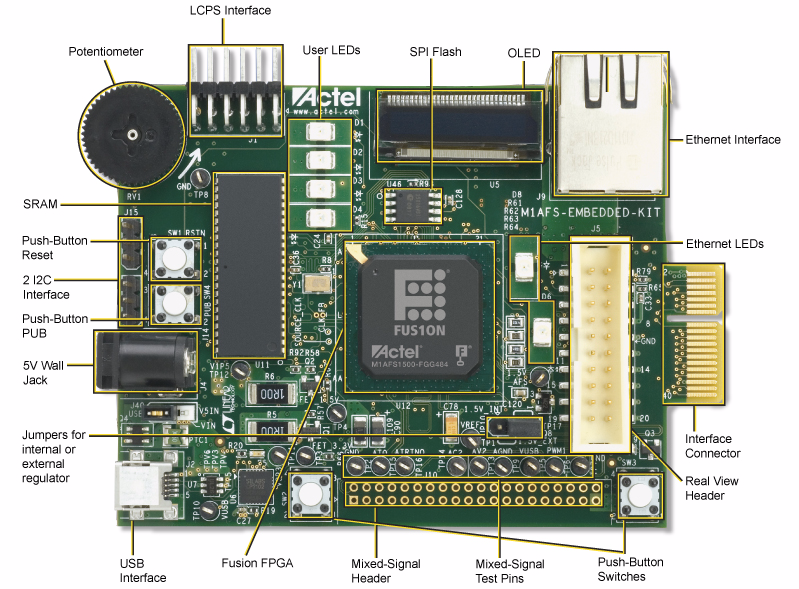
\includegraphics[width=0.8\textwidth]{devkit2}
	\caption[Actel Fusion Embedded Development Kit izstrādes platforma.]
			{Actel Fusion Embedded Development Kit izstrādes platforma \cite[7.~lpp.]{FusionGuide}.}
	\label{fig:devkit}
\end{figure}

Lai gan mikrokontroliera kodols ir izstrādāts platformas neatkarīgā VHDL,
parauga mikrokontroliera implementācija izmanto gan FPGA specifiskos
resursus, gan izstrādes platformas specifiskos resursus. Konkrēti, tika
izmantota uz izstrādes plates novietotā, 8 megabitu (512K mašīnvārdu)
ietilpības SPI \termEn{Flash} atmiņa \cite{FusionGuide}, kuras uzdevums ir uzglabāt 
pamatprogrammu (tās mašīnkodu).

Par darba vidi tika izmantota \textbf{Actel Libero IDE} programmpaka, kas
sevī iekļauj:
\begin{itemize}
	\item \textbf{Actel Libero} projekta pārvaldīšanai,
		kā arī HDL koda rediģēšanai un strukturālo komponenšu 
		grafisko shematiku zīmēšanai;
	\item \textbf{Mentor Graphics ModelSim} projekta darbības simulācijai
		un rezultātu (laika diagrammu) vizualizācijai;
	\item \textbf{Synopsis Synplify} projekta rezultāta sintēzei;
\end{itemize}

Papildus autors C un C++ valodā izstrādāja assembleri
 izstrādātā kodola instrukciju kopai mikrokontroliera mašīnkoda assemblēšanai.

	
	\clearpage
	\section{Bāzes prototipa analīze}
Šajā darbā izstrādātā mikrokontroliera kodols par paraugu izmanto
D.~Perija (\termEn{D.~Perry}) ,,VHDL: Programming by Example'' grāmatā
piedāvāto procesora imple\-men\-tā\-ciju \cite{Perry-VHDL}.

Sākotnēji (rev.~01) izstrādātais kodols izmantoja gandrīz identisku
arhitektūru (bet atšķirīgu instrukciju kopu), bet
jau agri izstrādes procesā tika identificētas vairāki arhitektūras trūkumi,
no kuriem daži padarīja prototipu nesintezējamu.
Šī nodaļa apskata šos trūkumus un piedāvātos risinājumus.
Problēmu risinājumi šajā nodaļā apskatīti visai virspusēji,
to implementācijas detaļas, pēc iestrādes kodolā,
sīkāk apskatītas \ref{sec:cpu}~un \ref{sec:uC}~nodaļā.

\begin{figure}[thb]
	\centering
	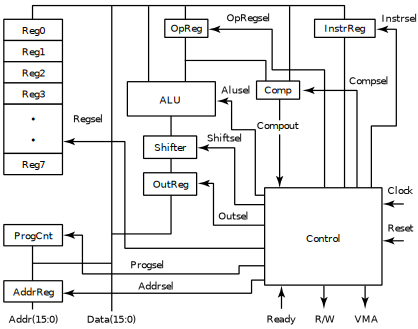
\includegraphics[scale=1.1]{perry-cpu}
	\caption[Bāzes prototipa uzbūves bloku diagramma.]
	        {Bāzes prototipa uzbūves bloku diagramma \cite[290.~lpp.]{Perry-VHDL}.}
	\label{fig:perry-cpu}
\end{figure}

D.~Perija procesors (turpmāk tekstā ,,bāzes prototips'')
ir vienkāršs 16 bitu procesors ar klasisku trīsstāvokļu 
centrālo datu šinu \cite{Flynn-arch}\cite{Heath}, un ar visām pamata
komponentēm (sk.~\ref{fig:perry-cpu}~att.), kas nodrošina bāzes prototipa
spēju izpildīt instrukcijas no tā instrukciju kopas.

\subsection{Iekšējā datu šina}
	Bāzes prototipa arhitektūra paredz kopēju, trīsstāvokļu iekšējo datu šinu
	(sk.~\ref{fig:perry-cpu}~att.).
	Šāda šinas uzbūve ir elektriski vienkārša, un ir shematiski viegli uztverama
	(sk.~\ref{fig:multidrop}~att.). Bet šāda uzbūve pieprasa šinas 
	,,arbitēšanu'', t.i.,~nepieciešams
	nodrošināt, ka tikai viena no šinai pievienotajām ierīcēm ir aktīvs devējs,
	kamēr pārējo ierīči izvadiem jābūt augstas impedances režīmā, kā arī
	jānodrošina lai pareizā ierīce (vai ierīces) šos datus nolasītu no šinas.

	\begin{figure}[thb]
		\centering
		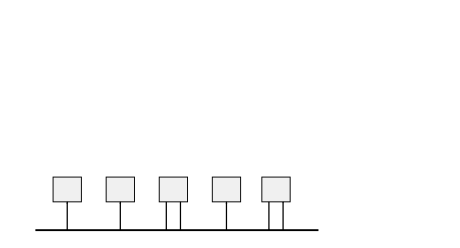
\includegraphics[scale=1.25]{multidrop}
		\caption{Kopējas trīstāvokļu datu šinas shēma.}
		\label{fig:multidrop}
	\end{figure}

	Galvenā problēma šādas šinas izmantošanai sintezējama kodola izstrādai ir
	fakts, ka vairums (vai pat visas) FPGA neatbalsta trīsstāvokļu
	loģiku, ko var secināt no fakta, ka neviena no apskatītajām FPGA neatbalsta
	loģisko bloku konfigurāciju ar atvērtā kolektora izejām
	\cite[18.~lpp.]{FusionFAQ}\cite{SmartFusionFabric}\cite{Xilinx7}.
	Tas nozīmē, ka pat ja sintēzes rīks atbalsta šādas šinas HDL aprakstu, tas
	ģenerēs ievērojami sarežģītāku struktūru, kas ,,emulē'' trīsstāvokļu datu šinu.

	Alternatīvas šinas uzbūvē ir ķēdes savienojumi vai maršrutējams tīkls.
	Maršrutējami tīklveida ir sarežģītas uzbūves, un pieprasa tikpat sarežģītu
	kontroles loģiku. Savukārt, ķēdes savienojumi ir pietiekami vienkārši,
	tādēļ tiek izvēlēti par risinājumu.

	\begin{figure}[thb]
		\centering
		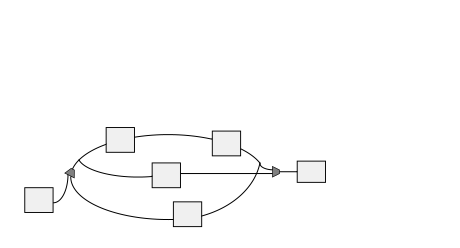
\includegraphics[scale=1.25]{chain}
		\caption{Vienvirziena cirkulāra ķēde ar atzarojumiem.}
		\label{fig:chain}
	\end{figure}

	Visai komplicēta ķēdes savienojumu struktūra ir redzama \ref{fig:chain}~attēlā,
	bet kas idejiski atbilst risinājuma rezultātam. 
	Ar ķēdes savienojumiem datu pārraide notiek vienā virzienā,
	tādējādi nav nepieciešamas bidirekcionālās pieslēgvietas, bet ir nepieciešamas
	atsevišķas pieslēgvietas datu ievadei un izvadei. Noslēdzot sazarojumus ar
	multipleksoriem arī zūd nepieciešamība pēc trīsstāvokļu loģikas.

	Ķēdes savienojumu priekšrocība ir arbitēšanas vienkāršums. Ierīces uz šinas
	jau ir savienotas ar datu saņēmejierīcēm, tādējādi vienīgā arbitēšana ir
	nodrošināt datu plūsmu (signalizēt datu nolasi) un sazarojumu noslēdzošo
	multipleksoru komutēšana.
	
	Ķēdes savienojumu šinas ieguvums ir arī tā potenciālais datu caurlaides
	apjoms (\termEn{troughput}), kas ir ievērojami lielāks, jo ierīces nav
	savienotas pie viena mezgla, kas kopējā datu šinā ir sastrēguma punkts
	(\termEn{bottleneck}). Datus dažādos ķēdes posmos var pārraidīt
	paralēli un šinas atzaru datu pārraides ātrums drīkst savā starpā 
	atšķirties.

	Tā kā procesora komponentēm nav nepieciešams komunicēt katrai ar katru, ir
	iespējams izveidot optimizētu kēžveida datu šinu, kur tieši savienotas ir tikai
	komponentes starp kurām notiek tieša komunikācija. Kodolā iestrādāto
	risināju skatīt \ref{sec:databus}~nodaļā.

\pagebreak[3]
\subsection{Instrukciju kopa}
	Bāzes prototips paredz vienkāršu instrukciju kopu, ar konstanta garuma
	5 bitu operāciju kodiem. Instrukciju kopa ir tipiska \termEn{Load/Store}
	principa procesoru arhitektūrām. \termEn{Load/Store} princips nosaka, ka
	visas aritmētiskās, loģiskās, bīdes un komparācijas darbības notiek
	ar vispārējā pielietojuma reģistru masīva reģistriem un datu apmaiņa ar
	operatīvo atmiņu notiek ar atmiņas nolases un ierakstes instrukcijām
	\cite[11.~lpp.]{Flynn-arch}	(sk.~\ref{sec:regArray}~nod.).
	Instrukcijas sadalāmas šādās grupās \cite[291.~lpp.]{Perry-VHDL}:
	\begin{itemize}
		\item \textbf{atmiņas nolases} (\termEn{load}) un \textbf{ierakstes}
			(\termEn{store}) instrukcijas, kuras
			veic datu apmaiņu starp reģistriem un operatīvo atmiņu;
		\item \textbf{zarošanās} instrukcijas, kas izmaina
			izpilāmā mašīnkoda (programmas) aktīvo pozīciju, un iekļauj
			nosacījuma un beznosacījuma zarošanās;
		\item instrukcijas, kuras veic \textbf{aritmētiskās} un 
			\textbf{bitu loģiskās} darbības ar reģistriem (operandiem);
		\item instrukcijas, kuras veic \textbf{bitu bīdes} reģistra
			(operanda) datiem.
	\end{itemize}
	
	Autorprāt, izmantotā instrukciju kopas izvēle ir racionāla, bet
	implementācija ir neoptimizēta. Pirmkārt, 5 bitu operācijas kods
	neefektīvi izmanto pieejamo 16 bitu mašīnvārdu
	(sk.~\ref{fig:5bit-opcode}~att.), un efektīvāk būtu izmantot mainīga
	garuma operācijas kodu.
	\begin{figure}[thb]
		\centering
		
\includegraphics[scale=1.25]{perry-instr}
		\caption[5 bitu operācijas koda instrukcijas vārds.]
		        {5 bitu operācijas koda instrukcijas vārds \cite[292.~lpp.]{Perry-VHDL}.}
		\label{fig:5bit-opcode}
	\end{figure}
	
	Otrkārt, bāzes prototipa instrukciju operāciju kodi nes tikai kontroles
	iekārtai nozīmīgu informāciju un tiek pilnībā dekodēti dekodēšanas solī.
	Tas nozīmē, ka katrai instrukcijai nepieciešami savi, unikāli stāvokļi
	kontroles iekārtā (kas realizēta kā stāvokļu mašīna). Tā kā piem., 
	aritmētiskās instrukcijas (\texttt{ADD}, \texttt{SUB}, utt.)
	tiek izpildītas praktiski vienādi, iespējams veikt daļēju operācijas
	koda dekodēšanu un deleģējot atlikušā operācijas koda ,,dekodēšanu''
	ALU (sk.~\ref{sec:alu}~nod.), nododot tai nozīmīgu informāciju no
	operācijas koda. Tādējādi tiek panākti viekāršāka dekodēšanas loģika un 
	mazāk stāvokļu kontroles iekārtā, jo pietiek ar vienu šablonveida
	izpildes stāvokļu ķēdi.
	
	Kodola realizācijai, autors ir pilnībā no jauna izveidojis instrukciju
	kopu, kas iekļauj visas iepriekš minētās instrukciju grupas, bet
	konkrētās instrukcijas un to izpildes implementācija, kas izmanto minētās optimizācijas,
	ievērojami atšķiras (sk.~\ref{sec:instrSet}~nod.).
	
	Izstrādājot kodolu arī veikta papildus, arhitektūras specifiska
	optimizācija. Gan bāzes prototipa (sk.~\ref{fig:perry-cpu}~att.),
	gan izstrādātā kodola (sk.~\ref{fig:cpu-rev3}~att.) uzbūvē ALU un
	,,bitu bīdes iekārta'' atrodas uz viena signālceļa, kas nozīmē, ka
	izpildot gan bīdes, gan aritmētiskās instrukcijas dati tiek pārvadīti
	caur abām ierīcēm. Šo arhitektūras īpašību var izmantot izveidojot
	instrukciju, kas var veikt abas operācijas vienlaicīgi.
	Šādi kodolā implementēta \mnem{AR} instrukcija (sk.~\ref{sec:AR}~nod.).
	Tas arī nozīmē, ka visas aritmētiskās un bīdes instrukcijas ir izsakāmas
	ar šo ,,šabloninstrukciju'' vēl vairāk vienkāršojot kontroles iekārtas
	dekodēšanas loģiku un instrukciju izpildes stāvokļus.
	
\subsection{Komparators} \label{sec:perry-comp}
	Bāzes prototipā izmantotais komparators (sk.~\ref{fig:perry-comp}~att.),
	kura uzdevums ir salīdzināt	divus operandus (|a| un |b|), izvada
	rezultātu (|compout|) atkarībā pēc salīdzināšanas režīma signāla uz |sel|
	\cite[309.~lpp.]{Perry-VHDL}.
	\begin{figure}[thb]
		\centering
		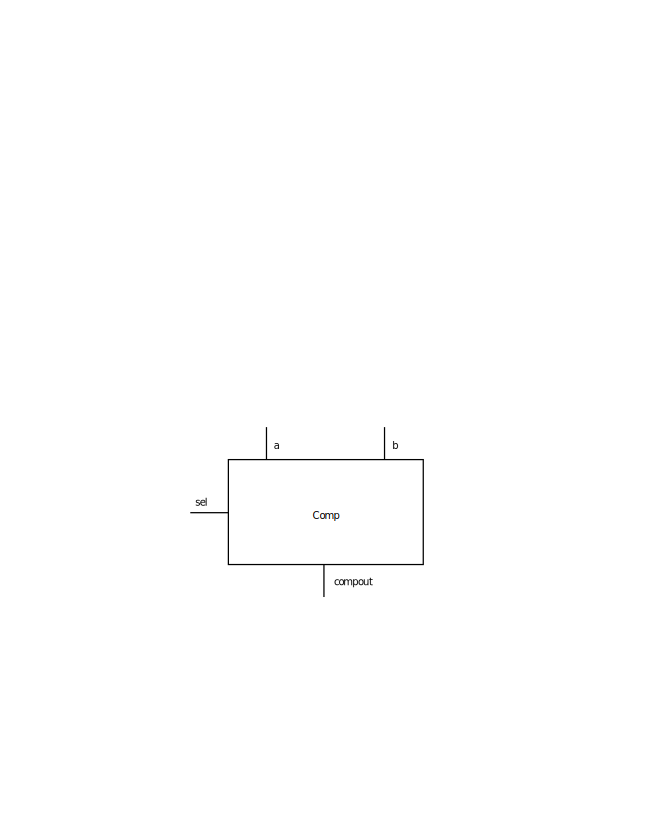
\includegraphics[scale=0.9]{perry-comp}
		\caption[Bāzes prototipa komparators.]
		        {Bāzes prototipa komparators \cite[309.~lpp.]{Perry-VHDL}.}
		\label{fig:perry-comp}
	\end{figure}
	
	Tiek definēti seši salīdzināšanas režīmi:
	\begin{itemize}
		\item operandu vienādība (|EQ|), kur |compout| ir |1|, ja |a|$=$|b|;
		\item operandu nevienādība (|NEQ|), kur |compout| ir |1|, ja |a|$\neq$|b|;
		\item operands |a| stingri lielāks (|GT|), kur |compout| ir |1|, ja |a|$>$|b|;
		\item operands |a| nestingri lielāks (|GTE|), kur |compout| ir |1|, ja |a|$\geq$|b|;
		\item operands |a| stingri mazāks (|LT|), kur |compout| ir |1|, ja |a|$<$|b|;
		\item operands |a| nestingri mazāks (|LTE|), kur |compout| ir |1|, ja |a|$\leq$|b|.
	\end{itemize}
	
	Šiem režīmiem eksistē ,,pretsakarības'', piem.~|EQ| ir pretējs |NEQ| un
	|GT| pretējs |LTE|, kas nozīmē ka šie režīmi ir redundanti. Izslēdzot
	redundantos režīmus iegūstam trīs: |LT|; |EQ|; |GT|, kas arī apzīmē
	trīs iespējamos operandu savstarpējos stāvokļus.
	Sekojot no matemātiskās aksiomas var pierādīt, ka
	\[
		\neg (a>b) \land (a \neq b) \iff (a<b)
	\]
	skaidri parādot, ka pārbaudot jebkurus divus stāvokļus trešais
	nosakāms pēc noklusējuma.
	\pagebreak[3]
	
	Tad tā vietā lai nodotu vienu no sešiem pārbaudes režīmiem,
	varam optimizēt, likvidējot režīmu pārslēgšanu vispār, un vienmēr izvadot
	rezultātu no divu operandu savstarpējo stāvokļu pārbaudes.
	
	Kodola realizācijā izmantots ,,bezrežīmu'' komparators, kas 
	divus signāla bitus, kas attiecīgi norāda 
	vai operands |a| ir vienāds ar |b|, 
	un vai operands |a| ir lielāks par |b| (sk.~\ref{sec:comp}~nod.).
	Protams šāda implementācija nozīmē papildus loģiku kontroles iekārtā,
	bet tās implementācija ir visai vienkārša, kā apskatīts
	\ref{sec:branching}~nodaļā.

%\subsection{Kontroles iekārta}
%	\todo

	
	% Praktiskā daļa
	\clearpage
	\section{Mikrokontroliera kodola realizācija} \label{sec:cpu}
	Mikrokontroliera kodols pēc savas būtības un uzbūves ir procesors,
	kurš veic kalkulācijas un datu apmaiņu, nodrošinot mikrokontroliera
	programmas izpildi.
	Šajā darbā izstrādātais mikrokontroliera kodols ir 
	Fon-Neimaņa (\termEn{von~Neumann}) arhitektūras pro\-ce\-sors, kurš
	izmanto 16 bitu instrukcijas%
		\footnote{Instrukcijas var būt $N$-skaita 16 bitu vārdi. 
		Šajā darbā realizētas viena un divu vārdu instrukcijas.}
	un 16 bitu atmiņas adreses. Arī atmiņas vienība, kurai pieder unikāla
	adrese, ir 16 bitu plata. Kā Fon-Neimaņa procesoram, datu un
	programmkoda atmiņa ir kopēja un vienādi adresējama.[\todo]
	
	Kodola uzbūve ir daļēji balstīta uz D.~Perija (\termEn{D.~Perry}) grāmatas%
	\cite{Perry-VHDL} piedāvāto procesora reali\-zā\-ciju, 
	bet ar ievērojamām izmaiņām, galvenokārt, pilnībā no jauna izstrādāta 
	instrukciju kopa un vienvirziena,
	cirkulāra datu apmaiņas šina, atšķirībā no kopējas,
	trīs\-stāvokļu arbitējamas datu šinas.
	Galvenais šādas uzbūves datu šinas realizācijas iemesls
	ir izmantojamās \termEn{Actel} FPGA darba platformas trīs\-stāvokļu
	loģikas atbalsta \mbox{trūkums.\cite[18.~lpp.]{FusionFAQ}}
	
	Kodola saskarne ar pārējām mikrokontroliera komponentēm ir izveidota
	pēc iespējas vienkāršāka un platformas neatkarīga, lai nebūtu nepieciešams
	veikt izmaiņas kodola uzbūvē izmantojot to dažādās mikrokontroliera
	implementācijās, t.i.~kodola datu apmaiņa notiek izmantojot
	asinhronu atmiņas (RAM)	saskarni. Ar dažādām ierīcēm iespējama
	komunikācija iespējama, ja tiek izmantota saskarnes komponente, kas
	emulē RAM un multipleksē perifērās iekārtas pēc nododamās adreses.
	Tādējādi kodols	ir praktiski neatkarīgs no pārējās 
	mikrokontroliera implementācijas.
	Šī īpašība izmantota mikrokontroliera paraugimplementācijā.
	(sk.~\ref{sec:design}~un \ref{sec:mmu}~nod.)
	% TODO: 
	
	Instruckiju kopa ir izstrādāta no jauna un piedāvā vienkāršotu,
	mini\-mālu kopu līdzīgi RISC (\termEn{Reduced Instruction Set Computing})
	filo\-so\-fijai. Salīdzinot ar Perija realizāciju, ievērojami samazinātas
	nosacījuma zarošanās instrukcijas un instrukcijas pieejamie 16 biti
	tiek efektīvāk izmantoti ieviešot vektorizētus jeb dažāda garuma
	operāciju kodus. (detalizētākam aprakstam sk.~\ref{sec:instrSet}~nod.)
	
	
	%Tā kā \termEn{Actel} FPGA risinājums neatbalsta trīs stāvokļu
	%loģiku\cite[18.~lpp.]{FusionFAQ},
	%tad kopēju iekšējo datu šinu nav iespējams
	%izveidot. Tā vietā izveidota vienvirziena, nosacīti cirkulāra datu
	%apmaiņas līnija. Datu līnijas sazarojumi dažādu komponenšu 
	%komunikācijai realizēti ar multipleksoru palīdzību.
	
	%\begin{figure}[bhp]
	%	\centering
	%	\def\svgwidth{\textwidth}
	%	{\ttfamily\scriptsize\input{img/control.pdf_tex}}
	%	\caption{Procesora kontrole un atmiņas saskarne.}
	%	\label{fig:controlPipeline}
	%\end{figure}
	%
	%\begin{figure}[thp]
	%	\centering
	%	\def\svgwidth{\textwidth}
	%	{\ttfamily\footnotesize\input{img/aluPipeline.pdf_tex}}
	%	\caption{Aritmētikas un loģikas signālceļš un uzbūve.}
	%	\label{fig:aluPipeline}
	%\end{figure}
	
	\begin{figure}[thb]
		\centering
		\def\svgwidth{\textwidth}
		{\ttfamily\footnotesize\input{img/top-rev3-detail.pdf_tex}}
		\caption{Kodola uzbūve.}
		\label{fig:cpu-rev3}
	\end{figure}
	
	%\pagebreak[4]
	%\clearpage
	% TODO: Atmiņas izdalījums, 'von Neumann bottleneck' un kā DMA palīdz
	\subsection{Iekšējās datu šinas uzbūve} \label{sec:databus}
Izveidotajam procesoram ir sazarota, cirkulāra datu apmaiņas šina atšķirībā no kopējas,
trīsstāvokļu arbitējamas datu šinas. Šādai šinas uzbūvei ir vairākas
priekšrocības:
\begin{description}
	\item[Nav trīsstāvokļu loģika] \hfill \\
		Trīsstāvokļu loģikas trūkums atbrīvo no nepieciešamības izmantot
		trīsstāvokļu komponentes procesora iekšējā uzbūvē,
		samazinot realizācijas kompleksitāti.
	\item[Elektriskā drošība] \hfill \\ %TODO: Šitam citādāku nosaukumu?
		Nevienai no komponentēm pie šinas nevar tikt savienotas izejas,
		likvidējot iespējamo kaitējumu arbitācijas kļūdu rezultātā.
	\item[Mazāk vadības signālu] \hfill \\
		Šādai implementācijai nav nepieciešami nolases un rakstīšanas
		vadības signālu pāri katrai pievienotai ierīcei. Vienvirziena datu
		apmaiņa ļauj tikai pievadīt rakstīšanas vadības signālu%
		\footnote{Lai uzsvērtu šo vadības signālu nozīmi reģistru satura
			atjaunošanā, to nosaukumiem pievienots -\texttt{Updt} piedēklis.}%
		, vai pat nevienu signālu kombinacionālo komponenšu gadījumā.
\end{description}

Viens no šādas šinas uzbūves trūkumiem var tikt uzskatīta nepieciešamība
multipleksēt signālus, bet pēc visu iespējamo datu apmaiņas scenāriju analīzes,
implementējamās instrukciju kopas ietvaros, tika noskaidrots ka --- 
pat ne tuvu --- katrai komponentei nepieciešama datu apmaiņa ar visām pārējām.
Konkrēti, tikai piecām komponentēm nepieciešama datu nolase no vairāk
nekā vienas citas.

%\todo % TODO: Tabula ar nepieciešamajiem savienojumiem
\begin{table}[hb]
	\centering
	\caption{Komponentes kurām nepieciešama ieejas multipleksēšana.}
	\label{tbl:muxes}
	\begin{tabular}{ll}
		\toprule
		Komponente & Ienākošie (multipleksējamie) dati\\ 
		\midrule
		Programmskaitītājs & Atmiņas ielase; ALU signālceļa dati\\
		Reģistru masīvs & Atmiņas ielase; ALU signālceļa dati\\
		ALU (pirmais operands) & Programmskaitītājs; Reģistru masīvs\\
		Komparators (pirmais operands) & Programmskaitītājs; Reģistru masīvs\\
		Adresācijas reģistrs & ALU signālceļa dati; Reģistru masīvs\\
		\bottomrule
	\end{tabular}
\end{table}

Apvienojot vienādos multipleksorus iegūstam optimizētu datu apmaiņas šinu
ar tikai trijiem \texttt{32>16} multipleksoriem. (sk.~\ref{fig:cpu-rev3}~att.)

%Galvenais šāda risinājuma iemesls
%ir izmantojamās \termEn{Actel} FPGA darba platformas trīs stāvokļu
%loģikas atbalsta \mbox{trūkums.\cite[18.~lpp.]{FusionFAQ}}
 %\clearpage 
	%\subsection{Procesora VHDL bibliotēka}
\todo
%\begin{singlespace}
	\lstinputlisting[language={[qucs]VHDL},float=h,%
					 caption={Procesora \texttt{cpu\_lib} pakas definīcija. (\texttt{cpu\_lib.vhd})},%
					 label=kb:cpulib,
					 basicstyle=\ttfamily\scriptsize]
		{code/cpu_lib.vhd}
%\end{singlespace}
	\clearpage
	\subsection{Komponentes}
Izstrādātais procesors (mikrokontroliera kodols) sastāv no vairākām
apakš\-kom\-po\-nentēm (sk.~\ref{fig:cpu-rev3}~att., \pageref{fig:cpu-rev3}~lpp.). 
Šo komponenšu uzbūve un darbība aprakstīta sintēzei
derīgā ,,RTL stila'' VHDL apraksta kodā izmantojot tikai standarta un
paša izveidotas pakotnes,
šādi panākot augstu implementācijas portabilitāti%
	\footnote{Iespējamu projekta izmantošanu dažādos izstrādes rīkos.}.
Lai izvairītos no ,,skriešanās problēmām'' (\termEn{race condition})
simulācijas laikā un arī simulētu signālu aizkavēšanos,
VHDL aprakstos visai bieži izmantota novēlotās piešķiršanas konstrukcija,
kuru sintēzes rīks ignorē.

Komponenšu VHDL aprakstos piesaukti tipi un konstantes no paša definētas
\texttt{cpu\_lib} pakotnes, kas redzama sekojošā koda blokā.
\begin{singlespace}
\lstinputlisting[language={[qucs]VHDL},%float=b,%
                 caption={Procesora \texttt{cpu\_lib} pakas definīcija (\texttt{cpu\_lib.vhd}).},%
                 label=kb:cpulib,basicstyle=\ttfamily\scriptsize]
	{code/cpu_lib.vhd}
\end{singlespace}
\pagebreak[3]

\FloatBarrier
\subsubsection{Reģistri}
	Viena no vienkāršākajām komponentēm ir reģistrs.
	Tā funkcija ir uzglabāt	viena mašīn\-vārdu datus 
	(šajā gadījumā 16 bitu vārda) un pārrakstīt to pēc
	pieprasījuma. Implementētais reģistrs ir sinhrons un dinamisks, un tā
	dati tiek pārrakstīti \texttt{clk} signālam pārejot no zema uz augstu
	stāvokli.
	\begin{figure}[bh]
		\centering
		%\def\svgwidth{7cm}
		\def\svgscale{1.25}
		{\ttfamily\scriptsize\input{img/sub-reg.pdf_tex}}
		\caption{Reģistrs.}
		\label{fig:reg}
	\end{figure}
	
	Reģistra VHDL apraksts ir visai triviāls un, ar nelielām izmaiņām
	(sk.~\ref{kb:reg}~pirmkodu),
	izmantots D.~Perija paraugs.\cite[321.~lpp.]{Perry-VHDL}
	%\begin{singlespace}
	% NOTE: No Need for singlespace when floated!
		\lstinputlisting[language={[qucs]VHDL},float=thb,%
		                caption={Reģistra VHDL apraksts. (\texttt{reg.vhd})},%
		                label=kb:reg]
			{code/reg.vhd}
	%\end{singlespace}
	
	\pagebreak[2]
	Lai gan reģistrs ir vienkārša ierīce, to plaši izmanto procesora
	realizācijā, uzglabājot ļoti dažādas nozīmes datus.
	Šī darba ietvaros izstrādātajā procesorā ir sekojoši speciālās nozīmes reģistri:
	\pagebreak[1]
	\begin{itemize}
		\item \textbf{Programmskaitītājs} (\texttt{PC}):
			Reģistrs, kas uzglabā adresi aktīvajai programmas pozīcijai,
			t.i.~parasti izpildāmās instrukcijas adresi. Secīgās programmas
			izpildes laikā \texttt{PC} tiek inkrementēts%
			\footnote{Konkrētāk — \texttt{PC} tiek palielināts par
				izpildīto instrukcijas vārdu skaitu (1 vai 2).},
			savukārt lēcieni (zarošanās)
			programmā realizēti pārrakstot programmskaitītāja saturu.\pagebreak[2]
		\item \textbf{Izpildāmās instrukcijas reģistrs} (\texttt{instrReg})
			ieraksta izpildāmās instrukcijas kodu.
			Nepieciešams, lai kontroles stāvokļa mašīna „neaizmirstu”
			izpildāmo operāciju un tās argumentus izpildot
			turpmākās mikro\-operācijas%
			\footnote{Mikrooperācijas ir soļi kas jāveic vienas instrukcijas
				izpildei. Kontroles iekārtas stāvokļi atbilst mikrooperācijām
				(sk.~kodu pielikumā \ref{appx:control}).}.
			Divu vārdu instrukcijām saglabāts
			tiek tikai pirmais vārds, jo tikai tajā ir dekodējamais
			operācijas kods. Otrais vārds satur tikai argumentus.
		\item \textbf{Atmiņas adresācijas reģistrs} (\texttt{addrReg})
			uzglabā adresējamo atmiņas adresi tās nolasei
			vai ierakstei. Nepieciešams, lai saglabātu adresi izpildot
			\mnem{LD} un \mnem{ST} instrukcijas (sk.~\ref{sec:instrSet}~nod.),
			%jo tikai viens no diviem iesaistītajiem operatīvajiem reģistriem
			jo tikai viens no diviem iesaistītajiem vispārējas nozīmes reģistriem
			(sk.~\ref{sec:regArray}~nod.) ir nolasāms vai pārrakstāms
			vienā mikrooperācijas solī.
		\item \textbf{Operanda reģistrs} (\texttt{opReg})
			uzglabā vienu no aritmētiskās/loģiskās darbības
			ope\-ran\-diem. Nepieciešams, jo ALU neuzglabā pievadītos
			operandus\footnote{ALU ir realizēta kā kombinacionāla shēma.}
			un abi operandi nolasāmi no tā paša datu avota.
			(par ALU sk.~\ref{sec:alu}~nod., \pageref{sec:alu}~lpp.)
		\item \textbf{Rezultāta reģistrs} (\texttt{outReg}),
			kurā ieraksta aritmētiskās/loģiskās darbības rezultātu.
			Tā kā ALU datu avots var būt (un parasti ir) arī rezultāta
			ierakstes mērķis, rezultāta reģistrs novērš 
			,,skriešanās problēmu'', kas būtu
			iespējama vienlaicīgi lasot un pārrakstot datu avotu.
	\end{itemize}

\pagebreak[3]
\FloatBarrier
%\subsubsection{Operatīvo reģistru masīvs}
\subsubsection{Vispārējas nozīmes reģistru masīvs} \label{sec:regArray}
	Vispārējas nozīmes reģistri ir reģistru kopa, kura, atšķirībā no
	iepriekš apskatītajiem procesora specializētajiem reģistriem,
	ir pieejama	programmētājam tiešai modifikācijai.
	Šiem reģistriem nav noteikta specializēta nozīme,
	tā vietā programmētājs tos lieto pēc vajadzības, piem.~izpildāmās
	programmas mainīgo uzglabāšanai.
	\begin{figure}[th]
		\centering
		%\def\svgwidth{7cm}
		\def\svgscale{1.25}
		{\ttfamily\scriptsize\input{img/sub-regArray.pdf_tex}}
		\caption{Reģistru masīvs.}
		\label{fig:regArray}
	\end{figure}
	
	Vispārējas nozīmes reģistru masīvs ir izpild\-programmas datu apstrādes
	krustpunkts. Tas ir tādēļ ka izstrādātais procesors, 
	līdzīgi vairumam RISC tipa arhi\-tek\-tūru,
	izmanto \termEn{Load/Store} principu, t.i.~visas aritmētiskās darbības
	tiek veiktas ar vispārējas nozīmes reģistriem un datu apmaiņa ar atmiņu (RAM)
	notiek tikai caur šiem reģistriem izmantojot datu apmaiņas
	instrukcijas\cite[11.~lpp.]{Flynn-arch}, šajā gadījumā \mnem{LD} un \mnem{ST}.
	
	%\begin{singlespace}
		\lstinputlisting[language={[qucs]VHDL},float=thb,%
		                caption={Reģistru masīva VHDL apraksts. (\texttt{regarray2.vhd})},%
		                label=kb:regArray,%
		                emph={t_ram}]
			{code/regarray2.vhd}
	%\end{singlespace}
	%\pagebreak[2]
	Realizācijā, kura redzama \ref{kb:regArray} pirmkoda blokā, 
	reģistru masīvs vairāk līdzinās 8 vārdu operatīvajai
	atmiņai, bet netiek realizēta rakstīšanas vai lasīšanas režīma
	pārslēgšana. Tā vietā ir ieejas un izejas pieslēgvietas un
	ierakstītie dati tiek saglabāti un uzreiz izlikti uz izvadi.
	
	Reģistru skaitu masīvā ierobežo pieejamais bitu skaits operācijas
	koda vārdā reģistra adreses\footnote{Vispārējas nozīmes reģistriem ir
		sava, neatkarīga adrešu telpa.}
 	uzglabāšanai. Konkrēti \mnem{AR} instrukcijai pieejami 3 biti reģistra
 	adresei, kas ierobežo vispārējās nozīmes reģistru skaitu līdz 8
 	(unikālo adrešu skaits 3 bitos).

\pagebreak[3]
\FloatBarrier
\subsubsection{Multipleksors}
	Multipleksors praktiski ir elektroniski kontrolēts ,,slēdzis'',
	kas pārslēdz divas vai vairāk ieejas uz vienu izeju. Ieejas un izejas
	ne obligāti ir viens signālvads (bits). Šajā gadījumā tiek pārslēgtas
	16 bitu platas datu maģistrāles, kur
	multipleksors tiek izmantots datu šinā, noslēdzot sazarojumu,
	lai pārslēgtu datu ieejas avotu aiz tā sekojošai komponentei
	(vai komponentēm).
	\begin{figure}[bhp]
		\centering
		%\def\svgwidth{7cm}
		\def\svgscale{1.25}
		{\ttfamily\scriptsize\input{img/sub-mux.pdf_tex}}
		\caption{2 ieeju multipleksors.}
		\label{fig:mux2}
	\end{figure}
	
	Multipleksors realizēts ar ļoti vienkāršu izejas vārda nosacījuma
	pārslēgšanu (sk.~\ref{kb:mux}~pirmkodu).
	%\begin{singlespace}
		\lstinputlisting[language={[qucs]VHDL},float=thb,%
		                 caption={Multipleksora VHDL apraksts (\texttt{mux.vhd}).},%
		                 label=kb:mux]
			{code/mux.vhd}
	%\end{singlespace}

\pagebreak[3]
\FloatBarrier
\subsubsection{Aritmētiski loģiskā ierīce} \label{sec:alu}
	Aritmētiski loģiskā ierīce jeb ALU ir viena no galvenajām
	procesora komponentēm. Tās uzdevums ir veikt doto datu apstrādi un,
	šī procesora realizācijā, arī
	palielināt programmskaitītāju secīgas programmas izpildes nodrošināšanai.
	\begin{figure}[thp]
		\centering
		%\def\svgwidth{7cm}
		\def\svgscale{1.25}
		{\ttfamily\scriptsize\input{img/sub-alu.pdf_tex}}
		\caption{Aritmētiski loģiskā ierīce.}
		\label{fig:alu}
	\end{figure}
	
	Lai gan klasiski bīdes operācijas arī tiek realizētas ALU,
	šajā gadījumā ALU veic tikai aritmētiskās un bitu
	loģikas darbības, atstājot bīdes operācijas „Bitu bīdes loģiskjai ierīcei”
	(sk.~\ref{sec:shifter}~nod.). Šāda sadalīšana ļauj veikt aritmētiskās
	un bīdes operācijas vienlaicīgi, uz ko balstās \mnem{AR} instrukcija
	(sk.~\ref{sec:AR}~nod.~\pageref{sec:AR}~lpp.).
	
	ALU realizēta kā kombinacionāla shēma ar asinhronu darbību,
	t.i.~izejas vērtība tiek izmainīta uzreiz,
	bez kontroles signāla (takts) pievadīšanas, un izejas vērtība ir tikai
	atkarīga no pievadīto operandu vērtībām, kuru vērtības iekšēji ALU
	netiek saglabātas.
	Lai būtu iespējams veikt darbības ar diviem
	operandiem no operatīvo reģistru masīva, tiek izmantots \texttt{opReg}
	reģistrs viena operanda uzglabāšanai, lai otru varētu nodot tieši.
	(sk.~\ref{fig:cpu-rev3}~att., \pageref{fig:cpu-rev3}~lpp.)
	
	\begin{singlespace}
		\lstinputlisting[language={[qucs]VHDL},%float=th,%
		                caption={ALU VHDL apraksts. (\texttt{alu.vhd})},%
		                label=kb:alu]
			{code/alu.vhd}
	\end{singlespace}
	
	ALU veic operācijas ar 16 bitu vārdiem, kuri reprezentē bezzīmes
	skaitļus. ALU VHDL implementācija izmanto \texttt{std\_logic\_unsigned}
	pakotnē	definētās aritmētiskās operācijas,
	ievērojami vienkāršojot ALU VHDL aprakstu (sk.~\ref{kb:alu}~pirmkodu).

\pagebreak[3]
\FloatBarrier
\subsubsection{Bitu bīdes loģiskā ierīce} \label{sec:shifter}
	Ierīce, kura šeit nosaukta par ,,Bitu bīdes loģisko ierīci'',
	realizē bitu bīdes operācijas, kuras šī procesora realizācijā ir
	izdalītas atsevišķi no ALU. 

	\begin{figure}[h!]
		\centering
		%\def\svgwidth{7cm}
		\def\svgscale{1.25}
		{\ttfamily\scriptsize\input{img/sub-shift.pdf_tex}}
		\caption{Bitu bīdes loģiskā ierīce.}
		\label{fig:shift}
	\end{figure}
	
	Realizācija, līdzīgi ALU, ir kombinacionāla un asinhrona. Ieejošie dati
	tiek pārbīdīti atkarībā pēc |sel| signāla stāvokļa 
	(sk.~\ref{kb:shifter}~pirmkodu).
	
	%\begin{singlespace}
		\lstinputlisting[language={[qucs]VHDL},float=th,%
		                caption={Bīdes ierīces VHDL apraksts. (\texttt{shifter.vhd})},%
		                label=kb:shifter]
			{code/shifter.vhd}
	%\end{singlespace}
	
	

%\clearpage
\pagebreak[3]
\FloatBarrier
\subsubsection{Komparators} \label{sec:comp}
	Komparators jeb salīdzinātājs ir komponente, kas salīdzina 
	divus operandus --- 16 bitu vārdus, kas tiek interpretēti kā bezzīmes
	skaitļi.
	Šī komparatora implementācija ir minimizēta, kombinacionāla un nesatur
	kontroles signālus (salīdzinājumam ar D.~Perry realizāciju sk.~\todo{}~nod.).
	Izvadīti tiek tikai divi loģiskie signāli, no kuriem |eq|
	norāda uz operandu vienādību (loģiskais |1|) vai nevienādību (loģiskā |0|),
	savukārt |gr| norāda vai operands \texttt{a} ir lielāks (|1|)
	par \texttt{b} vai nav (|0|). Ar šo
	informāciju ir pilnīgi pietiekami, lai būtu iepējams realizēt visas
	nosacījuma zarošanās (\mnem{BRxx}) instrukcijas
	(sk.~\ref{sec:branching}~nod.~\pageref{sec:branching}~lpp.).
	\begin{figure}[bhp]
		\centering
		%\def\svgwidth{7cm}
		\def\svgscale{1.25}
		{\ttfamily\scriptsize\input{img/sub-comp.pdf_tex}}
		\caption{Komparators.}
		\label{fig:comp}
	\end{figure}
	
	%\begin{singlespace}
		\lstinputlisting[language={[qucs]VHDL},float=thbp,%
		                %basicstyle=\ttfamily\scriptsize,%
		                caption={Komparatora VHDL apraksts. (\texttt{comp.vhd})},%
		                label=kb:comp]
			{code/comp.vhd}
	%\end{singlespace}

%\clearpage
%\FloatBarrier
\pagebreak[3]
\subsubsection{Kontroles iekārta} \label{sec:control}
	Viena no galvenajām procesora komponentēm ir kontroles iekārta, kas,
	iespējams, ir procesora sarežģītākā komponente. Kontroles iekārta
	nodrošina mikrooperāciju izpildi, kas kontrolē datu plūsmu starp
	procesora iekšējām komponentēm un datu apmaiņu ar RAM.
	\begin{figure}[hp]
		\centering
		%\def\svgwidth{7cm}
		\def\svgscale{1.1}
		{\ttfamily\scriptsize\input{img/sub-control.pdf_tex}}
		\caption{Kontroles iekārta.}
		\label{fig:control}
	\end{figure}
	
	Kontroles iekārta realizēta kā stāvokļa mašīna, kur katrs stāvoklis
	atbilst vienai mikrooperācijai, un, tātad, tās VHDL apraksts var tikt
	uzskatīts par analogu mikrokodam. Viena mikrooperācija tiek
	izpildīta vienā takts ciklā.
	
	Kontroles iekārta instrukcijas izpilda pa vienai, izdarot sekojošas
	soļus katras instrukcijas izpildē:
	\begin{enumerate}
		\item \textbf{instrukcijas ielase} (1 mikroop.) nolasa operācijas kodu no RAM
			un saglabā to turpmākai dekodēšanai;
		\item \textbf{instrukcijas dekodēšana} (1 mikroop.) pēc operācijas
			koda nosaka nepieciešamās mikrooperācijas konkrētai instrukcijas
			izpildei; %\footnote{Konkrēti tikai jānosaka viena nākamā izpildāmā
				%mikrooperācija, jo aiz tās sekojošas mikroop.~izpildās jau
				%noteiktā kārtībā};
		\item \textbf{datu ielase un operācijas izpilde} (0--7 mikroop.)
			veic instrukcijas specifiskās operācijas, kas var iekļaut
			nevienu, vienu vai vairākas no sekojošām operācijām:
			\begin{itemize}
				\item datu ielase no RAM;\footnote{%
					Datu nolase var aizņemt vairākus takts ciklus līdz
					atmiņa ir gatava datu pārraidei (\texttt{ready} tiek pacelts).}
				\item datu ierakste RAM;
				\item aritmētiskā un/vai bīdes operācija;
				\item zarošanās nosacījuma pārbaude;
				\item programmskaitītāja pārrakstīšana zarošanās izpildei;
			\end{itemize}\pagebreak[1]
		\item \textbf{programmskaitītāja inkrementācija} veic sagatavošanos
			nākamās instrukcijas izpildes ciklam.
	\end{enumerate}
	
	Kontroles iekārtas kods ir pārāk apjomīgs un komplicēts, lai to
	apskatītu šeit, tādēļ atsevišķas tā daļas tiks izskatītas turpmākajās
	nodaļās un pilnais kods iekļauts pielikumā~\ref{appx:control}
 \pagebreak[3]
	\subsection{Instrukciju kopa} \label{sec:instrSet}
%Instruckiju kopa ir izstrādāta no jauna un piedāvā vienkāršotu,
%mini\-mālu kopu līdzīgi RISC (\termEn{Reduced Instruction Set Computing})
%filo\-so\-fijai. Salīdzinot ar Perija realizāciju, ievērojami samazinātas
%nosacījuma zarošanās instrukcijas un instrukcijas pieejamie 16 biti
%tiek efektīvāk izmantoti ieviešot vektorizētus jeb dažāda garuma
%operāciju kodus. (detalizētākam aprakstam sk.~\ref{sec:instrSet}~nod.)

Instruckiju kopa ir izstrādāta no jauna un piedāvā vienkāršotu kopu, kas
satur pamata darbības ar bezzīmes veseliem (\texttt{unsigned integer} tipa)
skaitļiem, RAM ielasīšanas un ierakstes instrukcijas, un zarošanās
instrukcijas (sk.~\ref{tbl:instructions}~tabulu).

Instrukcijas operāciju kodi ir dažāda garuma, jeb vektoriski\footnote{%
	Termins aizgūts no programmēšanas paņēmiena, kur viena funkcija
	satur dažādu operāciju kopu (vektoru), un pēc nodotā argumenta tiek
	izpildīta viena operācija (mainot pārējo argumentu nozīmi).},
t.i.~operāciju kods sadalīts ,,grupas'' kodā un ,,vektora'' kodā, kur
grupas kods ir konstanta garuma (2~biti), bet vektora kods ir konstanta
garuma tikai piederošās grupas ietvaros. Strikti ņemot, varētu uzskatīt, ka
vektora kods ir arguments, bet uzskatāms par piederīgu operācijas
kodam, jo abas tā daļas tiek interpretētas dekodēšanas solī.\footnote{%
	Izņemot \mnem{AR} instrukciju (sk.~\ref{sec:AR}~nod.).}

\begin{singlespace}\small
\begin{longtable}[c]{lp{20ex}lp{0.36\textwidth}}
	%\centering
	\caption{Instrukciju tabula.}\label{tbl:instructions}\\
	\toprule
	\textbf{Apz.} & \textbf{Mašīnkods} & \textbf{Argumenti} & \textbf{Operācija} \\
	\midrule \endfirsthead
	\caption[]{\nameref{tbl:instructions}~(turpinājums).}\\
	%\toprule
	\midrule
	\textbf{Apz.} & \textbf{Mašīnkods} & \textbf{Argumenti} & \textbf{Operācija} \\
	\midrule \endhead
	\multicolumn{4}{c}{Atmiņas datu apmaiņas instrukcijas}\\
	\midrule
	\mnem{LD} & 	\instr{01}{00}{}{XXXXXX}{XXX}{XXX}{} & \texttt{rD, rS} &
		\texttt{rD = *(rS)} \newline
		{\footnotesize Ielasa vārdu no RAM reģistrā \texttt{rD}} \\ \midrule
	\mnem{LDI} & 	\instr{01}{01}{}{XXXXXX}{XXX}{}{XXX} \newline
					\instr{}{}{}{}{}{XXXXXXXXXXXXXXXX}{} & \texttt{rD, C} &
		\texttt{rD = C} \newline
		{\footnotesize Ielasa konstanti reģistrā \texttt{rD}} \\ \midrule
	\mnem{ST} & 	\instr{01}{11}{}{XXXXXX}{XXX}{XXX}{} & \texttt{rD, rS} &
		\texttt{*(rD) = rS} \newline
		{\footnotesize Ielasa vārdu no RAM reģistrā \texttt{rD}} \\
	\midrule \pagebreak[3]
	\multicolumn{4}{c}{Aritmētikās, loģikās un bitu bīdes instrukcijas (un \mnem{AR} operācijas saīsnes)}\\
	\midrule
	\mnem{AR} & 	\instr{10}{}{}{}{XXXX}{XXX}{X}\instr{}{}{}{}{XXX}{XXX}{} & \texttt{kA, kS, rD, rS} &
		{\footnotesize Aritmētikas/bīdes instrukcija.} \\ \midrule
	\rule{0pt}{1em}\mnem{ADD} & \instr{10}{0000}{000}{X}{XXX}{XXX}{} & \texttt{rD, rS} &
		\verb|rD = rD + rS| \\ \midrule
	\rule{0pt}{1em}\mnem{SUB} & \instr{10}{0001}{000}{X}{XXX}{XXX}{} & \texttt{rD, rS} &
		\verb|rD = rD - rS| \\ \midrule
	\rule{0pt}{1em}\mnem{INC} & \instr{10}{1000}{000}{X}{XXX}{}{XXX} & \texttt{rD} &
		\verb|rD = rD + 1| \\ \midrule
	\rule{0pt}{1em}\mnem{DEC} & \instr{10}{1001}{000}{X}{XXX}{}{XXX} & \texttt{rD} &
		\verb|rD = rD - 1| \\ \midrule
	\rule{0pt}{1em}\mnem{AND} & \instr{10}{0010}{000}{X}{XXX}{XXX}{} & \texttt{rD, rS} &
		\verb|rD = rD & rS| \\ \midrule
	\rule{0pt}{1em}\mnem{OR} & \instr{10}{0011}{000}{X}{XXX}{XXX}{} & \texttt{rD, rS} &
		\verb+rD = rD | rS+ \\ \midrule
	\rule{0pt}{1em}\mnem{XOR} & \instr{10}{0100}{000}{X}{XXX}{XXX}{} & \texttt{rD, rS} &
		\verb|rD = rD ^ rS| \\ \nopagebreak \midrule
	\rule{0pt}{1em}\mnem{NOT} & \instr{10}{1010}{000}{X}{XXX}{}{XXX} & \texttt{rD} &
		\verb|rD = ~rD| \\ \midrule
	\rule{0pt}{1em}\mnem{CLR} & \instr{10}{1111}{000}{X}{XXX}{}{XXX} & \texttt{rD} &
		\verb|rD = 0| \\ \midrule
	\rule{0pt}{1em}\mnem{MOV} & \instr{10}{0101}{000}{X}{XXX}{XXX}{} & \texttt{rD, rS} &
		\verb|rD = rS| \\ \midrule
	\rule{0pt}{1em}\mnem{LSL} & \instr{10}{0101}{001}{X}{XXX}{XXX}{} & \texttt{rD} &
		\verb|rD = rS * 2| \newline
		{\footnotesize loģiskā kreisā bīde (reizina ar 2)} \\ \midrule
	\rule{0pt}{1em}\mnem{LSR} & \instr{10}{0101}{010}{X}{XXX}{XXX}{} & \texttt{rD} &
		\texttt{rD = rS / 2} \newline
		{\footnotesize loģiskā labā bīde (dala ar 2)} \\ \midrule
	\rule{0pt}{1em}\mnem{ROL} & \instr{10}{0101}{011}{X}{XXX}{XXX}{} & \texttt{rD} &
		{\footnotesize bitu rotācija pa kreisi} \\ \midrule
	\rule{0pt}{1em}\mnem{ROR} & \instr{10}{0101}{100}{X}{XXX}{XXX}{} & \texttt{rD} &
		{\footnotesize bitu rotācija pa labi} \\ \nopagebreak
	\midrule \pagebreak[3]
	\multicolumn{4}{c}{Plūsmas kontroles instrukcijas}\\
	\midrule
	\mnem{NOP} & 	\instr{00}{}{}{00000000000000}{}{}{} & nav &
		{\footnotesize tukša operācija} \\ \midrule
	\mnem{HLT} & 	\instr{11}{0011}{}{XXXX}{}{}{XXXXXX} & nav &
		{\footnotesize apstādina procesora darbību} \\ \midrule
	\mnem{JMP} & 	\instr{11}{0010}{}{XXXX}{}{}{XXXXXX} \newline
					\instr{}{}{}{}{XXXXXXXXXXXXXXXX}{}{} & \texttt{L} &
		\texttt{PC = L} \newline
		{\footnotesize beznosacījuma lēciens.} \\ \midrule
	\mnem{BREQ} & 	\instr{11}{1000}{}{XXXX}{XXX}{XXX}{} \newline
					\instr{}{}{}{}{XXXXXXXXXXXXXXXX}{}{} & \texttt{rD, rS, L} &
		\texttt{if(rD==rS) PC = L} \\ \midrule
	\mnem{BRNQ} & 	\instr{11}{1011}{}{XXXX}{XXX}{XXX}{} \newline
					\instr{}{}{}{}{XXXXXXXXXXXXXXXX}{}{} & \texttt{rD, rS, L} &
		\texttt{if(rD!=rS) PC = L} \\ \midrule
	\mnem{BRGT} & 	\instr{11}{1010}{}{XXXX}{XXX}{XXX}{} \newline
					\instr{}{}{}{}{XXXXXXXXXXXXXXXX}{}{} & \texttt{rD, rS, L} &
		\texttt{if(rD>rS) PC = L} \\ \midrule
	\mnem{BRGE} & 	\instr{11}{1001}{}{XXXX}{XXX}{XXX}{} \newline
					\instr{}{}{}{}{XXXXXXXXXXXXXXXX}{}{} & \texttt{rD, rS, L} &
		\texttt{if(rD>=rS) PC = L} \\ \midrule
	\mnem{BRLT} & 	\multicolumn{2}{c}{subst.~\texttt{\textbf{BRGE} rS, rD, L}} &
		\texttt{if(rD<rS) PC = L}\\ \midrule
	\mnem{BRLE} & 	\multicolumn{2}{c}{subst.~\texttt{\textbf{BRGT} rS, rD, L}} &
		\texttt{if(rD<=rS) PC = L}\\
	\bottomrule
	\caption*{\fboxrule=0.75pt \framebox{\footnotesize
		\begin{tabular}{ll}
			\multicolumn{2}{c}{Mašīnkoda krāsu apzīmējumi} \\
			\textcolor{purple}{\rule[-2pt]{1em}{1em}} Operāciju grupas kods &
			\textcolor{blue}{\rule[-2pt]{1em}{1em}} \textcolor{cyan}{\rule[-2pt]{1em}{1em}}
				Operācijas vektora kods \\[2pt]
			\textcolor{lightgray}{\rule[-2pt]{1em}{1em}} Ignorētie biti &
			\textcolor{OliveGreen}{\rule[-2pt]{1em}{1em}} \textcolor{Green}{\rule[-2pt]{1em}{1em}}
				Argumentu biti \\
		\end{tabular}
		}}
\end{longtable}
\end{singlespace}
\normalsize

%\pagebreak
Instrukcijas
ir sadalītas grupās vai nu pēc nozīmes, vai pēc izpildes līdzības. Šo
instrukciju realizācijas detaļas tiks apskatītas turpmākajās apakšnodaļās.

\subsubsection{\mnem{AR} instrukcija} \label{sec:AR}
	Lai gan \mnem{AR} instrukcijas apzīmējums ir saīsinājums no „aritmētika”
	un tā ir instrukcijas primārā nozīme, \mnem{AR} implementē visas
	aritmētiskās, loģiskās, bīdes operā\-cijas, kā arī reģistru 
	apmaiņas \mnem{MOV} instrukciju (sk.~\ref{tbl:instructions}~tabulu).
	Šāda imple\-men\-tā\-cija izmantota tāpēc, ka visas šīs instrukcijas tiek
	pārvadītas pa to pašu signālceļu. Tādējādi kontroles iekārta tiek
	vienkāršota, jo atsevišķās operācijas nav nepieciešams izšķirt.
	
	Kontroles signāli aritmētiskajai un bīdes ierīcei,
	kā argumenti jeb vektora kodi,
	tiek nodoti tieši no instrukcijas vārda, un kontroles iekārtā netiek
	interpretēti (jeb ir „necaurspīdīgi”). Izņēmums, gan ir vektora koda
	vecākais bits, kurš tiek interpretēts un pie augsta stāvokļa (loģiskā |1|)
	tiek apieta otrā operanda (\texttt{rS}) ielase samazinot nepieciešamo
	takts ciklu skaitu instrukcijas izpildei (sk.~\ref{kb:ARdecode}~koda bloku).
	Šis bits ir |1|	unārājām un bezargumentu instrukcijām
	\mnem{INC}, \mnem{DEC}, \mnem{NOT} un \mnem{CLR}.%
	\footnote{Instrukcijas \mnem{LSL}, \mnem{LSR}, \mnem{ROL} un \mnem{ROR}
		nav īsti unāras, bet asemblējot šīs saīsnes izmanto to argumentu gan kā
		\texttt{rS}, gan kā \texttt{rD}.}
	
	\begin{singlespace}
		\lstinputlisting[language={[qucs]VHDL},%float=pb,%
		                caption={\mnem{AR} instrukcijas dekodēšana (izgriezums).},%
		                label=kb:ARdecode,%
		                firstnumber=150]
			{code/gen/ardecode-snippet.vhd}
	\end{singlespace}
	
	\mnem{AR} instrukcijas saīsnes nenosedz visas iespējamās darbības, kuras
	iespējamas ar \mnem{AR}. Tā kā ALU un Bitu bīdes loģiskā ierīce ir
	atsevišķas komponentes uz viena signālceļa, tās darbības ir izpildāmas
	vienlaicīgi. Tādējādi, izmantojot \mnem{AR} pilno formu, iespējams
	kombinēt aritmētiskās un bīdes operācijas (piem. saskaitīt un veikt bīdi)
	izpildei vienā instrukcijā. Jāņem vērā, ka Bitu bīdes loģiskā ierīce
	atrodas aiz ALU (sk.~\ref{fig:cpu-rev3}~att.),
	tādēļ bitu bīde vienmēr tiek izpildīta aritmētiskās darbības rezultātam.


\subsubsection{Nosacījuma zarošanās instrukcijas} \label{sec:branching}
	Nosacījuma zarošanās ir vitāla īpašība procesoram. Programmēšanas
	valodu \texttt{if()} konstrukcija nav iedomājama bez
	nosacījuma zarošanās.
	
	Izstrādātais procesors par zarošanās nosacījumu var izmantot divu reģistru
	satura apzīmēto bezzīmes veselo skaitļu salīdzinājumu.
	Šai salīdzināšanai atbilst \mnem{BRxx} instrukcijas
	(sk.~\ref{tbl:instructions}~tabulu), un pašu salīdzināšanu veic komparators
	(sk.~\ref{sec:comp}~nod.) kuram tiek pievadīti salīdzināmie operandi.
	
	\pagebreak[2]
	Aparatūras līmenī realizētas četras zarošanās instrukcijas:
	\begin{itemize}
		\item \mnem{BREQ} — zaroties, ja operandi ir vienādi;
		\item \mnem{BRNQ} — zaroties, ja operandi nav vienādi;
		\item \mnem{BRGE} — zaroties, ja pirmais operands ir lielāks
			vai vienāds ar otro;
		\item \mnem{BRGT} — zaroties, ja pirmais operands ir stingri lielāks
			par otro.
	\end{itemize}
	
	Zarošās nosacījumā pārbaudei tiek izmantoti šo instrukciju operāciju
	kodu divi jaunākie biti, kuri turpmāk šajā nodaļā apzīmēti ar
	\texttt{A} (otrs jaunākais bits) un \texttt{B} (jaunākais bits).
	
	Šo četru instrukciju operāciju kodi nav izvēlēti gluži patvaļīgi,
	bet pielāgoti tā, lai to \texttt{A} un \texttt{B} biti,
	kopā ar komparatora signāliem |eq| un |gr|
	(apz.~\texttt{E} un \texttt{G}),
	veidotu pēc iespējas vienkāršāku loģisko izteiksmi,
	kas izsaka zarošanās nosacījuma izpildi (sk.~\ref{fig:branch-karnaugh}~att.).
	
	\begin{figure}[thp]
		\centering
		%\def\svgwidth{7cm}
		\def\svgscale{1.5}
		{\ttfamily\input{img/karnaugh.pdf_tex}}\\
		\(
			f = \mathtt{\overline{A}E + BG + AG + AB\overline{E}}
		\)\\ %[1ex]
		%(apzīmējumu nozīmi sk.~\ref{kb:branchTest}.~kodā)
		\caption{Zarošanās nosacījuma Karno karte un formula.}
		\label{fig:branch-karnaugh}
	\end{figure}
	
	Zarošanās nosacījuma pārbaude implementēta kontroles iekārtā kā
	VHDL funkcija (sk.~\ref{kb:branchTest}~pirmkodu).
	
	\begin{singlespace}
		\lstinputlisting[language={[qucs]VHDL},%float=pb,%
		                caption={Zarošanās nosacījuma pārbaudes funkcija (izgriezums).},%
		                label=kb:branchTest,%
		                linerange={61-69},firstnumber=61,
		                emph={state,branchTest},%
		                breaklines,breakatwhitespace,
		                basicstyle=\ttfamily\scriptsize]
			{code/control2.vhd}
	\end{singlespace}
	
	Atlikušās zarošanās instrukcijas \mnem{BRLT} un \mnem{BRLE} ir
	programmatūras līmeņa substitūcijas, jo to ekvivalentus var iegūt
	izmantojot attiecīgi \mnem{BRGE} un \mnem{BRGT} instrukcijas,
	apmainot salīdzināmos operandus vietām assemblēšanas brīdī.
	
	
 %\clearpage %\pagebreak[3]
	% Man vajag revīziju cēsturi?
	%\subsection{Revīziju vēsture} \label{sec:cpu-revs}
%\todo

\begin{description}
	\item[Rev.~01] \hfill \\
		Par pamatu ņemta Perija grāmatas\citeet{Perry-VHDL} procesora
		realizācija. Atsevišķas komponentes izveidotas ļoti līdzīgi, bet
		kontroles iekārtas modelis un tam piekārtotā instrukciju tabula
		pilnībā izstrādāta no jauna.
	\item[Rev.~02] \hfill \\
		\termEn{Actel Fusion} FPGA nepiedāvā trīs-stāvokļu loģiku.\citeet{FusionFAQ}
		Tā rezultātā
		datu apmaiņas šina, pārveidota no kopējas arbitējamas 
		\termEn{multidrop} realizācijas pārveidota uz sazarotu vienvirziena
		pārraides ķēdi. Šāds solis pavildus ļāva arī likvidēt trīs-stāvokļu
		buferus un samazināt kontroles iekārtas signālu skaitu.
	\item[Rev.~03] \hfill \\
		Šī revīzija nav ienesusi fundamentālu izmaiņu procesora uzbūvē.
		(Izmaiņas sistēmas perifērijā skatīt
			\ref{sec:sys-revs}.~nod.~\pageref{sec:sys-revs}.~lpp.)
\end{description}
 %\pagebreak[3]
	
	% TODO?: Programmskaitītāja lokācija un PIC kods
 % Kodola uzbūve perifērija
	
	\clearpage
	\section{Sistēmas perifērija}
	Atsevišķs procesors ir nefunkcionāls, ja tam nevar pievadīt izpildāmās
	instrukcijas, atgūt datus vai vadīt kādu citu perifēro ierīci.
	
	Praktiski vienmēr procesoram nepieciešama atmiņas iekārta (RAM), kur
	glabāt izpildāmo programmu, kā arī pirmsapstrādes, pēcapstrādes un 
	apstrādes laika datus.
	
	Šajā nodaļā apskatītas divas sistēmas shēmas, no kurām viena veiksmīgi
	nosimulēta, bet nav sintezējama (rev.~02) un krietni sarežģītākā
	sintezējamā shēma, kura satur papildus perifērās ierīces.
	
	\subsection{Simulētā shēma (rev.~02)}
Sākotnējā darba augšējā līmeņa sistēmas gala shēma paredzēta, kā
paškomplektējoša, tikai ar procesoru un atmiņu, 
kur no ārpuses tiek tikai dota takts (\texttt{CLOCK})
un atiestatīšanas signāls ($\overline{\texttt{RESET}}$). Darbības pārbaudei
tiek izmantotas izstrādes platformas piedāvātās diodes.

\begin{figure}[bhp]
	\centering
	\def\svgwidth{\textwidth}
	{\ttfamily\tiny\input{img/top-rev2.pdf_tex}}
	\caption{Augšējā līmeņa shēma (rev.~02).}
	\label{fig:top-rev2}
\end{figure}

Šī shēma tika veiksmīgi simulēta pirms sintēzes
(rezultātus sk.~\ref{appx:simulation}.~pielikumā),
bet tā nav korekti sintezējama, jo paredz RAM sākotnējos datus,
kurus sintēzes rīks ignorē.
Realitātē RAM dati tiek pazaudēti tikko tiek noņemts barošanas spriegums un
tātad pēc šādas shēmas nav iespējams saglabāt izpildāmo programmu.

\pagebreak[3]
%\subsubsection{Operatīvā atmiņa}
	Operatīvā atmiņa šeit realizēta ar divām vienvirziena datu apmaiņas
	šinām. Kontroles signāli izmantoti līdzīgi klasiskai trīs-stāvokļu
	divvirzienu datu šinas atmiņai, pielāgojoties procesora atmiņas
	saskarnei.
	
	\begin{singlespace}
		\lstinputlisting[language={[qucs]VHDL},%float=p,
		                caption={RAM VHDL entītija.},%
		                label=kb:ram-entity,%
		                linerange={7-13},firstnumber=7,
		                breaklines,breakatwhitespace]
			{code/mem.twoport.vhd}
	
		\lstinputlisting[language={[qucs]VHDL},%float=p,
		                caption={RAM VHDL arhitektūras apraksts (izgriezums).},%
		                label=kb:ram-trimmed,%
		                linerange={85-99},firstnumber=85,%
		                breaklines,breakatwhitespace]
			{code/mem.twoport.vhd}
	\end{singlespace}
	
	\noindent Pilno kodu skatīt \ref{appx:ram-code}.~pielikumā.
 \clearpage %\pagebreak[3]
	\subsection{Papildinātā shēma (rev.~03)}
Šī apakšnodaļa apraksta sistēmas papildinājumus funkcionālas, sintezējamas
sistēmas realizācijai. Šīs revīzijas implementācija \textbf{nav pabeigta},
tādēļ šī apakšnodaļa ir uzskatāma par \textbf{turpmākā darba dokumentāciju},
nevis realizētu implementāciju.

Trešā sistēmas revīzija pievieno patstāvīgās atmiņas elementus sākotnējās
programmas un datu uzglabāšanai. Šīs atmiņas ierīces piekārtotas kopējai
adresācijas telpai, tādējādi rodas nepieciešamība pēc adreses dekodēšanas
loģikas, kuru nodrošina MMU (\termEn{Memory map unit}).



\subsubsection{Boot ROM}
	\termEn{Boot ROM} ir tikai nolasāmā atmiņa, kura paredzēta
	\termEn{bootstrap} procesa programmas uzglabāšanai.
	Šīs programmas uzdevums ir ielādēt reālo izpildes programmu no
	patstāvīgās atmiņas — šajā implementācijā konkrēti 
	no SPI \termEn{Flash} atmiņas.
	
	Par \termEn{Boot ROM} kalpos \termEn{Actel Fusion} piedāvātais
	\termEn{FlashROM} makross.\citeet{FlashROM}
	Maksimāli pieejamais ROM garums uz izmantojamās platformas ir
	1 kilobits jeb 64 vārdi.\citeet{FusionGuide}

\subsubsection{Adrešu telpai piekārtotā ievade/izvade}
	Papildus adresācijas telpā tiks piekārtoti speciālie reģistri dažādu
	perifēro ierīču datu apmaiņai un konfigurācijai.
	
	Uz doto brīdi (un kā redzams blokshēmā — \ref{fig:top-rev3}.~att.)
	paredzēta tikai SPI saskarne. Tam paredzēts viens pārraides un viens
	konfigurācijas reģistrs. Tam paredzēta iespēja nokonfigurēt datu
	apmaiņu pa baitam (8 biti) vai pa vārdam (16 biti). Datu pārraide tiek
	uzsākta uzreiz pēc jauno datu ierakstes reģistrā (ja SPI iespējots) un
	tiek pārraidīti bez procesora līdzdalības.
	
	\begin{figure}[thp]
		\centering
		%\def\svgwidth{7cm}
		\def\svgscale{1.25}
		{\ttfamily\scriptsize\input{img/sub-spi.pdf_tex}}
		\caption{SPI saskarnes ierīce.}
		\label{fig:spi}
	\end{figure}
	
	SPI saskarne nepieciešama komunikācijai ar SPI \termEn{Flash} atmiņu,
	kura pieejama uz izstrādes platformas,\cite[43.~lpp.]{FusionGuide}
	kur tiks glabāta galvenā izpildāmā programma, kura \termEn{boot} procesa
	laikā tiks pārvietota uz RAM.

\subsubsection{MMU — adrešu dekoderis} \label{sec:mmu}
	MMU jeb adrešu dekoderis ir ierīce, kas atbild par adrešu telpas
	pārdalīšanu dažādām ierīcēm, kā arī nodrošināt korektu komunikāciju
	ar šīm ierīcēm.
	
	\begin{figure}[thp]
		\centering
		\def\svgwidth{0.75\textwidth}
		{\ttfamily\small\input{img/remap.pdf_tex}}
		\caption{Adrešu telpas sadalījums.}
		\label{fig:memory-map}
	\end{figure}
	
	MMU tādējādi ar procesoru veido tādu pašu saskarni kā RAM un aparatūras
	līmenī ir pilnībā „caursīdīga”, savukārt piekārtojamo ierīču saskarne
	ir implementācijas definēta.
	
	\termEn{Boot ROM} nepieciešams piekārtot ar sākumu adresē \texttt{0x0000},
	lai pēc atiestatīšanas procesors sāktu izpildīt \termEn{boot} programmu.
 \clearpage %\pagebreak[3]
	\subsection{Revīziju vēsture} \label{sec:sys-revs}
%\todo

\begin{description}
	\item[Rev.~01] \hfill \\
		Kā RAM izmantota atmiņas realizācija ar 
		trīs-stāvokļu, divvirzienu datu šinu.
	\item[Rev.~02] \hfill \\
		Līdzīgi revīzijas izmaiņām procesora uzbūvē, arī atmiņa pārveidota,
		likvidējot trīs-stāvokļu šinu un tā vietā divas vienvirziena šinas
		datu ieejai un izejai. Kontroles signāli atstāti bez izmaiņām,
		tādējādi atmiņa vēljoprojām „emulē” trīs-stāvokļu datu apmaiņu,
		saglabājot procesora iespēju strādāt ar divvirzienu šinas atmiņu
		(papildus izmantojot virziena maiņas buferus).
	\item[Rev.~03] \hfill \\
		Šī revīzija veic fundamentālas izmaiņas sistēmas perifērijā,
		pievienojot patstāvīgo atmiņu un realizējot adrešu telpas
		piekārtošanu datu ievades/izvades ierīcēm ar MMU palīdzību.
		Šai arī paredz sistēmas \termEn{boot} procesu, kur izpildes
		programma tiek pārvietota izpildei uz operatīvo atmiņu no
		patstāvīgās atmiņas.
\end{description}

 % Sistēmas perifērija
	
	\clearpage
	\section{Secinājumi}

% 1: FPGA ir kruts jo iespeejams sintezeet HDL aprakstus

% Vaig RJMP

	
	% Literatūras saraksts
	\bibliographystyle{ieeetr}
	%\renewcommand{\refname}%
	%	{\vspace*{-12mm}\section*{Izmantotā literatūra}\vspace*{-6mm}}
	\clearpage
	%\pagestyle{empty}
	{\raggedright
	\begin{thebibliography}{99}
		\addcontentsline{toc}{section}{\refname}
		\bibitem{VHSIC}
			Creasey~D.J.,
			\textit{Advanced Signal Processing}.\linebreak[1]
			London: Peter~Peregrinus, 1985. ISBN~0-86341-037-5
		
		\bibitem{Flynn-arch}
			%Michael J.~Flynn,
			Flynn~M.J.,
			\textit{Computer Architecture: Pipelined and Parallel Processor Design}.
			\linebreak[3]
			London: Jones~and~Bartlett, 1995. ISBN~0-86720-204-1
		
		\bibitem{Golshan-ASIC}
			%Steve Heath,
			Golshan~K.,
			\textit{Physical Design Essentials: An ASIC Design Implementation Perspective}.
			New York: Springer, 2007. ISBN~0-387-36642-3
		
		\bibitem{Heath}
			%Steve Heath,
			Heath~S.,
			\textit{Embedded systems design}, 2\nd edition.\linebreak[3]
			Oxford: Newnes, 2003. ISBN~0-7506-5541-1
		
		\bibitem{VITAL}
			IEEE,
			\textit{IEEE 1076.4/D1, DRAFT Standard, VITAL ASIC Modeling Specification}.
			New York: IEEE, 2000.
		
		\bibitem{ieee-1364.1}
			IEEE,
			\textit{IEEE Std. 1364.1-2002, IEEE Standard for Verilog Register Transfer Level Synthesis}.
			New York: IEEE, 2002.
		
		\bibitem{HDL}
			%Gaurav Mehta, Sridhar Kintali,
			Mehta~G., Kintali~S.,
			\textit{Hardware Description Languages}.\linebreak[2]
			Santa Barbra: University of California,
			2009.
		
		%\bibitem{von-Neumann}
		%	John von Neumann,
		%	\textit{First Draft of a Report on the EDVAC},\linebreak[2]
		%	University of Pennsylvania, 1945.
		
		\bibitem{Perry-VHDL}
			%Douglas L.~Perry,
			Perry~D.L.,
			\textit{VHDL: Programming by Example}, 4\nth edition. \linebreak[2]
			New York: McGraw-Hill, 2002. ISBN~0-07-140070-2
		
		\bibitem{Vivek-Verilog}
			%Vivek Sagadeo,
			Sagdeo~V.,
			\textit{The Complete Verilog Book}.\linebreak[2]
			Norwell: Kluwer Academic Publishers, 1998. ISBN~0-7923-8188-2
		
		\bibitem{Vahid-RTL}
			%Frank Vahid,
			Vahid~F.,
			\textit{Digital Design with RTL Design, VHDL, and Verilog}, 2\nd edition.\linebreak[2]
			New York: % Hell knows which city
			John Wiley \& Sons, 2011. ISBN~978-0-470-53108-2
		
		\bibitem{FusionGuide}
			Actel corp.,
			\textit{Fusion Embedded Development Kit User's Guide}. %\linebreak[2]
			%USA: Actel,
			2009.
		
		\bibitem{FlashROM}
			Actel corp.,
			\textit{Fusion FlashROM}, Application Note AC236. %\linebreak[2]
			%USA: Actel,
			2005.
		
		\bibitem{RAM4K9}
			Actel corp.,
			\textit{Fusion SRAM/FIFO Blocks}, Application Note AC237. %\linebreak[2]
			%USA: Actel,
			2005.
		
		\bibitem{FusionFAQ}
			Actel corp.,
			\textit{Synplify — Synthesis Frequently Asked Questions}. %\linebreak[2]
			%USA: Actel,
			2009.
		
		\bibitem{SmartFusionFabric}
			Microsemi corp.,
			\textit{SmartFusion FPGA Fabric User's Guide}.
			%USA: Microsemi,
			2011.
		
		\bibitem{Xilinx7}
			Xilinx,
			\textit{7 Series FPGAs Overview}.
			%USA: Xilinx,
			2012.
		
		\bibitem{Mealy-VHDL}
			%Bryan Mealy, Fabrizio Tappero,
			Mealy~B., Tappero~F.,
			\textit{Free Range VHDL}.
			2012. [tiešsaiste] \linebreak[2]
			Pieejams: \url{http://www.freerangefactory.org/dl/free_range_vhdl.pdf}\linebreak[2]
			\mbox{[skatīts on 2012.~gada 2.~maijā]}
		
		\bibitem{vhdl-vs-verilog}
			Smith~D.J.,
			\textit{VHDL \& Verilog Compared \& Contrasted}. [tiešsaiste]\linebreak[2]
			Pieejams: \url{http://www.angelfire.com/in/rajesh52/verilogvhdl.html}
			\mbox{[skatīts on 2012.~gada 21.~maijā]}
		
		\bibitem{Kumar-Verilog}
			% Deepak Kumar Tala,
			Tala~D.K., \textit{Gate Level Modeling}. [tiešsaiste]\linebreak[2]
			Pieejams: \url{http://www.asic-world.com/verilog/gate.html}
			\mbox{[skatīts on 2012.~gada 24.~maijā]}
	\end{thebibliography}
	} % "End of \raggedright"
	
	\clearpage
	\begin{center}
	\phantomsection\addcontentsline{toc}{section}{Galvojums}
	\Large\bfseries Galvojums
\end{center}

Ar šo es, Jānis Šmēdiņš, galvoju, ka bakalaura darbs ir izpildīts patstāvīgi,
konsultējoties ar darba vadītāju. No svešiem pirmavotiem ņemtā informācija
ir norādīta ar atsaucēm, dati un definējumi ir uzrādīti darbā.
Šis darbs tādā vai citādā veidā nav nekad iesniegts nevienai
citai pārbaudījumu komisijai.

\vspace{3cm}
\noindent
\begin{minipage}{\textwidth}
	\raggedright
	2012.~gada \textcolor{gray}{\rule[-2pt]{2em}{1pt} \rule[-2pt]{10em}{1pt}}
	\hfill
	\textcolor{gray}{\rule[-2pt]{10em}{1pt}}\\[-1ex]
	\hfill\makebox[10em][c]{\tiny (paraksts)}
\end{minipage}

	
	\clearpage
	%\phantomsection\addcontentsline{toc}{section}{\appendixtocname}
	%\appendix
	\begin{appendices} % Pielikumu sākas šeit
	%\addappheadtotoc
	%\appendixtocname % Pievienot vārdu 'Pielikums' pie numura
	\addappheadtotoc
\begin{subappendices}
	\renewcommand\thefigure{\Alph{subsection}.\arabic{figure}}
	\renewcommand\thetable{\Alph{subsection}.\arabic{table}}
	\subsection{Eksperimenta protokols: FAST CPU implementāciju salīdzinājums}\label{appx:test1}
\setcounter{table}{0} %Reset table counter for (sub)appendix
\setcounter{figure}{0} %Reset figure counter for (sub)appendix
Eksperimenta mērķis ir salīdzināt
eksistējošo FAST algoritma implementāciju ātrdarbību CPU platformai, 
dodot iespēju izvērtēt implementācijas detaļas vadoties 
pēc kvantitatīva rādītāja. Iegūtie rezultāti arī uzstāda ātrdarbības 
,,etalonu'' GPU un FPGA platformu implementācijām.

Eksperiments tika veikts uz vairākiem datoriem, kuru aprīkojums norādīts
\ref{tbl:test1-dev}~tabulā. Izmantotie datori nosedz vairākas procesoru
sēriju paaudzes, kā arī reprezentē dažādas veiktspējas ,,spektra'' daļas.
\begin{table}[hb]\footnotesize
	\centering
	\caption{Izmantotās iekārtas (datori).}
	\label{tbl:test1-dev}
	\vspace{4pt}
	\begin{tabular}{cllll}
		\toprule
		\textbf{Nr.} & \textbf{Procesors} & \textbf{Takts frekvence} & 
			\textbf{Operētājsistēma} & \textbf{Arhitektūra}\\
		\midrule
		I & AMD Phenom 9950 & 2.60 GHz & Linux 3.10.7 (Gentoo) & \texttt{x86\_64}\\
		II & Intel Pentium M 740 & 1.73 GHz & Linux 3.10.17 (Gentoo) & \texttt{x86}\\
		III & Intel Core i5-2430M & 2.40 GHz & Windows 7 (+cygwin) & \texttt{x86\_64}\\
		IV & AMD Phenom II X6 1150T & 2.80 GHz & Linux 3.8.0 (Ubuntu) & \texttt{x84\_64}\\
		\bottomrule
	\end{tabular}
\end{table}

\begin{table}[hb]\footnotesize
	\centering
	\caption{Ātrdarbības rezultāti.}
	\label{tbl:test1-data}
	\vspace{4pt}
	\begin{tabular}{clcccrr}
		\toprule
		\input{results1-t1.tbl_tex}
		\bottomrule
	\end{tabular}
\end{table}
\footnotetext[1]{Kadri sekundē (angļu \termEn{frames per second}).}
\footnotetext{Miljoni pikseļu sekundē.}

Par ieejas datiem tika izmantota ,,\termEn{bas-relief}'' attēlu kopa%
	\footnote{Pieejama no \url{http://www.edwardrosten.com/work/junk.tar}},
kuru Rostens~un~Dramonds\cite{FAST} izmantoja FAST atkārtojamības testiem.
Uzstādītais jutības slieksnis $t$ visos testos bija 25, un katra 
attēla, iekārtas un implementācijas testa permutācija tika atkārtota 10 reizes.
Lielā datu apjoma dēļ (600 ieraksti) visa kopa netiek atspoguļota. Datu
apkopojums redzams \ref{tbl:test1-data}~tabulā, kur ,,Vid.~max'' kolonna
atspoguļo augstāko vērtību no kopas attēlu vidējiem rādītājiem
(t.i., ,,grūtākā'' kopas attēla vidējais apstrādes laiks 10 mērījumos).
,,Min'' un ,,Max'' kolonnas atspoguļo attiecīgi absolūto minimumu un absolūto
maksimumu no (80) uzņemto mērījumu sērijas.

\begin{figure}[tbh]
	\centering
	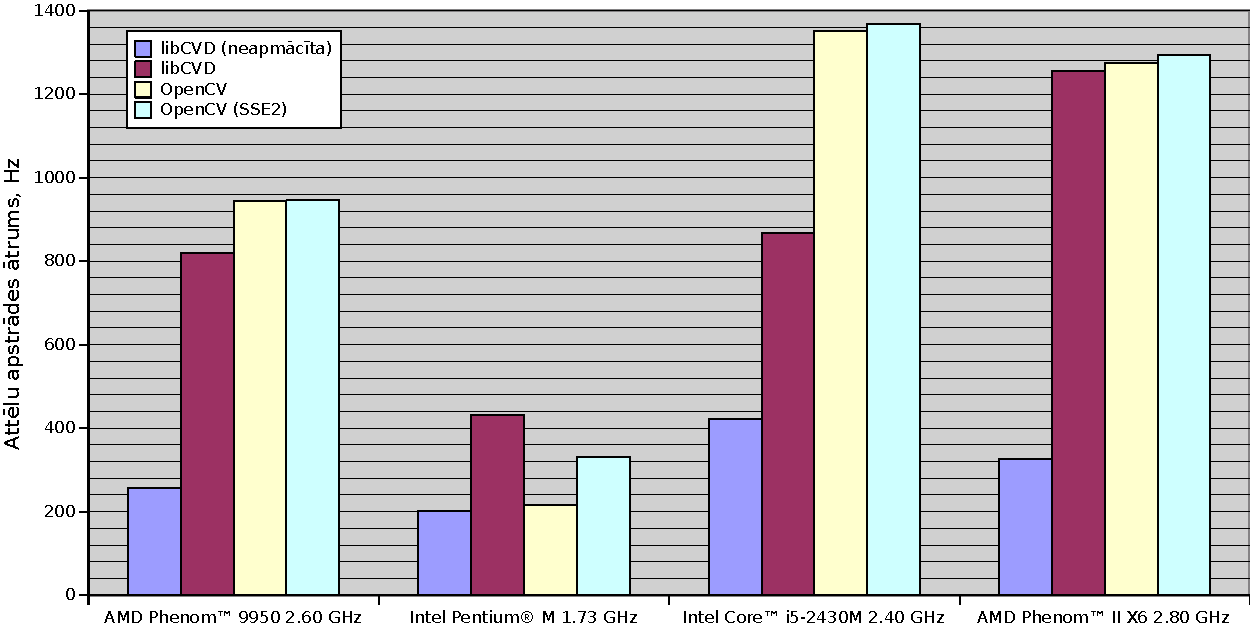
\includegraphics[width=\linewidth]{chart-cpu}
	\caption{Ātrdarbība dažādām implementācijām dažādās ierīcēs.}
	\label{fig:test1-data}
\end{figure}

Apskatot rezultātus (\ref{tbl:test1-data}~tabulu vai \ref{fig:test1-data}~attēlu)
ir veicami vairāki interesanti novērojumi. Lai gan CVD un OpenCV implementāciju
ātrdarbības uzlabojums pār neapmācīto CVD versiju bija paredzēts, to
savstarpējās atšķirības ir neparedzēti nekonsistentas.

Pirmkārt, CVD bibliotēkas implementācijas ātrdarbība ir augstāka uz vecas
paaudzes Pentium, bet jaunāko paaudžu procesoriem to pārspēj OpenCV
implementācija. Autors spekulē, ka OpenCV implementācijai ar tās LUT 
(\termEn{look-up table}) ir priekšroka
jauno paaudžu procesoros, to lielākas \termTech{kešatmiņas} dēļ, kas var saglabāt
visu LUT un attēla gabalu zemākā \termTech{kešatmiņas} līmenī, un, iespējams,
arī ātrākas atmiņas instrukciju izpildes dēļ. Šīs atšķirības iemesliem
nepieciešama papildus izpēte.

Otrkārt, OpenCV SSE2 versija sniedz tikai minimālus uzlabojumus ierīcēm
I, III un IV. Pēc papildus analīzes konstatēts, ka GCC kompilators,
pēc noklusējuma, 64~bitu sistēmām, iespējo SSE un SSE2 optimizāciju,
neatkarīgi no to atspējošanas ,,CMake'' vidē.
Tādējādi ,,neoptimizētā OpenCV'' rezultāti
šīm ierīcēm nav uzskatāmi par korektiem, un SSE2 uzlabojuma
salīdzināšanai nepieciešams testu atkārtot ar atspējotu SSE2 optimizāciju
kompilatora līmenī.

	\clearpage\subsection{Eksperimenta protokols: FAST FPGA resursu patēriņš un veiktspēja}\label{appx:test3}
\setcounter{table}{0} %Reset table counter for (sub)appendix
\setcounter{figure}{0} %Reset figure counter for (sub)appendix
Eksperimenta mērķis ir novērtēt potenciālo izvirzītā FAST algoritma FPGA modeļa
implementācijas ātrdarbību noskaidrojot resursu patēriņu 
konkrētai parauga FPGA mērķa platformai.
Par parauga FPGA tika izvēlēts Xilinx Virtex-6 (\texttt{XC6VLX75T}), % 6vlx75tff484-3
kuram programmējums tika sintezēts ar Xilinx XST rīku.

\begin{table}[hb]\footnotesize
	\centering
	\caption{FPGA modeļa resursu lietojums un ātrdarbība.}
	\label{tbl:test3-data}
	\vspace{4pt}
	\begin{tabular}{*{7}{c}}
		\toprule
		\input{fpga_test-t1.tbl_tex}
		\bottomrule
	\end{tabular}
	\begin{minipage}{0.5\linewidth}
		\noindent Apzīmējumi:\\
		$N_F$ --- \texttt{fast\_n\_unit} entītijas instanču skaits\\
		$f_\text{clk}$ --- takts frekvence\\
		$B_\text{in}$ --- nepieciešamā datu ieejas caurlaidspēja
	\end{minipage}
\end{table}
\footnotetext{Miljoni pikseļu sekundē.}

Eksperimentā tika sintezēti FAST attēla gabala apstrādes vienības
(\texttt{fast\_n\_chunk\_processor} entītijas) varianti ar pieaugošu
apstrādājamā attēla gabala laukumu. Rezultāti apkopoti
\ref{tbl:test3-data}~tabulā un attēloti \ref{fig:test3-data}~attēlā.
Maksimālā frekvence tika koriģēta, pēc
signālceļa garākās aiztures, jo tika konstatēts, ka sintēzes rīks,
visticamāk nekorekti, noteica maksimālo frekvenci $430.793\units{MHz}$
neatkarīgi no \texttt{fast\_n\_unit} instanču skaita.
\ref{fig:test3-data}~attēlā koriģētie rezultāti attēloti ar tumši zilo
grafiku un (salīdzināšanai) nekoriģētie ar gaiši zilu.

Jāņem vērā, ka sintēzes rezultāti par izmantotajiem resursiem un signāla izplatīšanos
(t.sk.,~maksimālo takts frekvenci) ir tikai aptuvens novērtējums, jo iegūti
pirms ,,resursu izvietošanas'' (\termEn{place and route}) soļa.
Autors uzskata, ka iegūtie dati ir pilnībā adekvāti,
ņemot vērā, ka rezultāti ir paredzēti tikai priekšstata radīšanai par
potenciālo ātrdarbību FPGA platformai.

\begin{figure}[tbh]
	\centering
	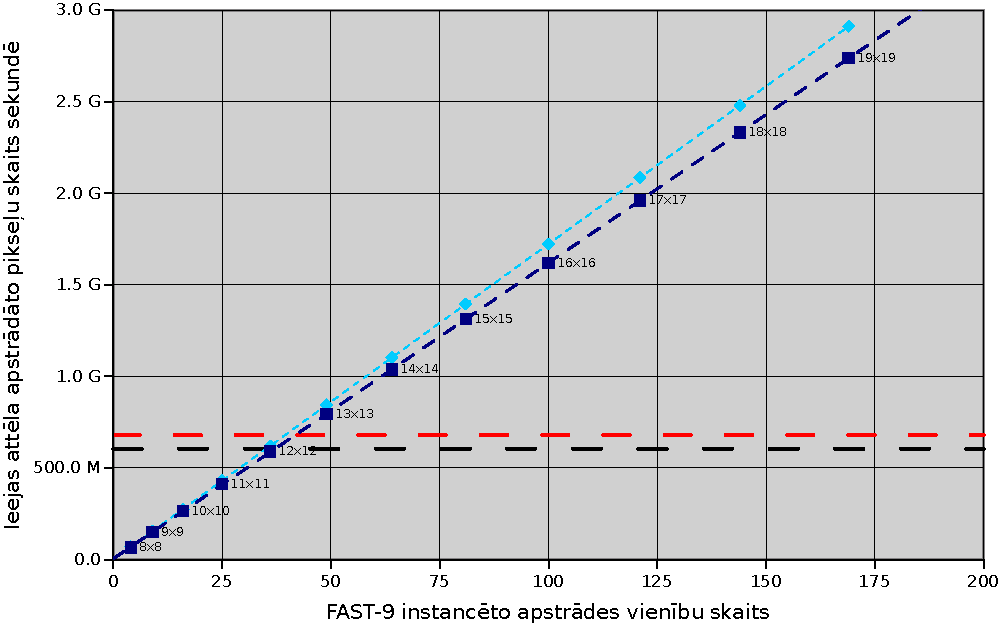
\includegraphics[width=0.9\textwidth]{chart-fpga}
	\caption{Pikseļu apstrādes ātrums pret \texttt{fast\_n\_unit} instanču skaitu.}
	\label{fig:test3-data}
\end{figure}

Pēc rezultātiem var novērot, ka $12 \times 12$ pikseļu gabala apstrāde pie
aptuveni $400\units{MHz}$ takts frekvences sasniedz labākos iegūtos
ātrdarbības rezultātus CPU platformai
(atzīmēts \ref{fig:test3-data}~attēlā ar pārtrauktu, melnu līniju)
izmantojot tikai ceturtdaļu FPGA resursu. Tomēr, lai gan FPGA resursu pietiek
skaitļošanas veiktspējas palielināšanai, šī veiktspēja nav izmantojama, jo
ātrdarbību ierobežo Virtex-6 ātrākās saskarnes (PCI~Express~v2.0~x8)
caurlaidspēja: 20~Gbps (atzīmēts \ref{fig:test3-data}~attēlā ar pārtrauktu,
sarkanu līniju). Var secināt, ka skaitļošanas kompleksitāte salīdzinājumā
ar ieejas datu apjomu nav pietiekami liela, lai panāktu būtisku uzlabojumu
pār CPU. Jānorāda, ka papildus skaitļošana būs nepieciešama raksturpunktu
deskriptoru izveidei un salāgošanai, ko pievienojot ir sagaidāma lielāks
ātrdarbības uzlabojums, jo CPU veiktspēja samazināsies papildus skaitļošanas
dēļ, bet FPGA vēl ir pieejami resursi un papildus skaitļošanu varēs veikt
paralēli FAST algoritmam.

\end{subappendices}

	\end{appendices}
	
	\clearpage
	\vspace*{2cm}\raggedright
\thispagestyle{empty}
Bakalaura darbs aizstāvēts Gala pārbaudījumu komisijas sēdē\\[1cm]
2012.~gada \textcolor{gray}{\rule[-2pt]{3em}{1pt}\hspace{1ex}\rule[-2pt]{10em}{1pt}}\\[1em]
un novērtēts ar atzīmi \textcolor{gray}{\rule[-2pt]{10em}{1pt}}\\[1em]

\vspace{2cm}
\noindent Protokols Nr. \textcolor{gray}{\rule[-2pt]{3em}{1pt}}\\[1cm]

\noindent
Gala pārbaudījumu komisijas priekšsēdētājs\\[1cm]
\textcolor{gray}{\rule[-2pt]{20em}{1pt}}\\[-1ex]
\makebox[20em][c]{\tiny (paraksts)}


	
	
\end{document}
